\section{Optical ultrasonic detection (OUSD)}
\label{sec:OUSD}
The requirements towards the setups in photoacoustic microscopy, shown in figure \ref{fig:ORPAMsetup}, have in common that the ultrasonic transducer has to be placed as close as possible to the origin of the ultrasonic wave. In order to achieve such configurations it is necessary to drill holes through the piezo-electric transducer or bypass the ultrasonic wave or excitation light to minimize the loss of information. Another approach to this topic is to use light, to detect ultrasonic waves and therefore combine optical and acoustical pathways. 

\subsection{Principle of optical ultrasonic detection}

The approach is based on a Fabry–P\'{e}rot interferometer (FPI). In a FPI light is applied onto two partially transmitting mirrors, which are placed parallel to each other. This setup is called resonator because only wavelengths that meet a certain resonance condition are transmitted through it.\\
The operation principle of the FPI based OUSD is shown in figure \ref{fig:transmissionChange}. In order to get a measurable signal of  a pressure wave running through the resonator, a medium is placed between the mirrors, which changes its refractive index due to pressure. This leads to a variation of the resonance condition.

\begin{figure}[H]
	a)
	\begin{minipage}{0.5\textwidth}
		
		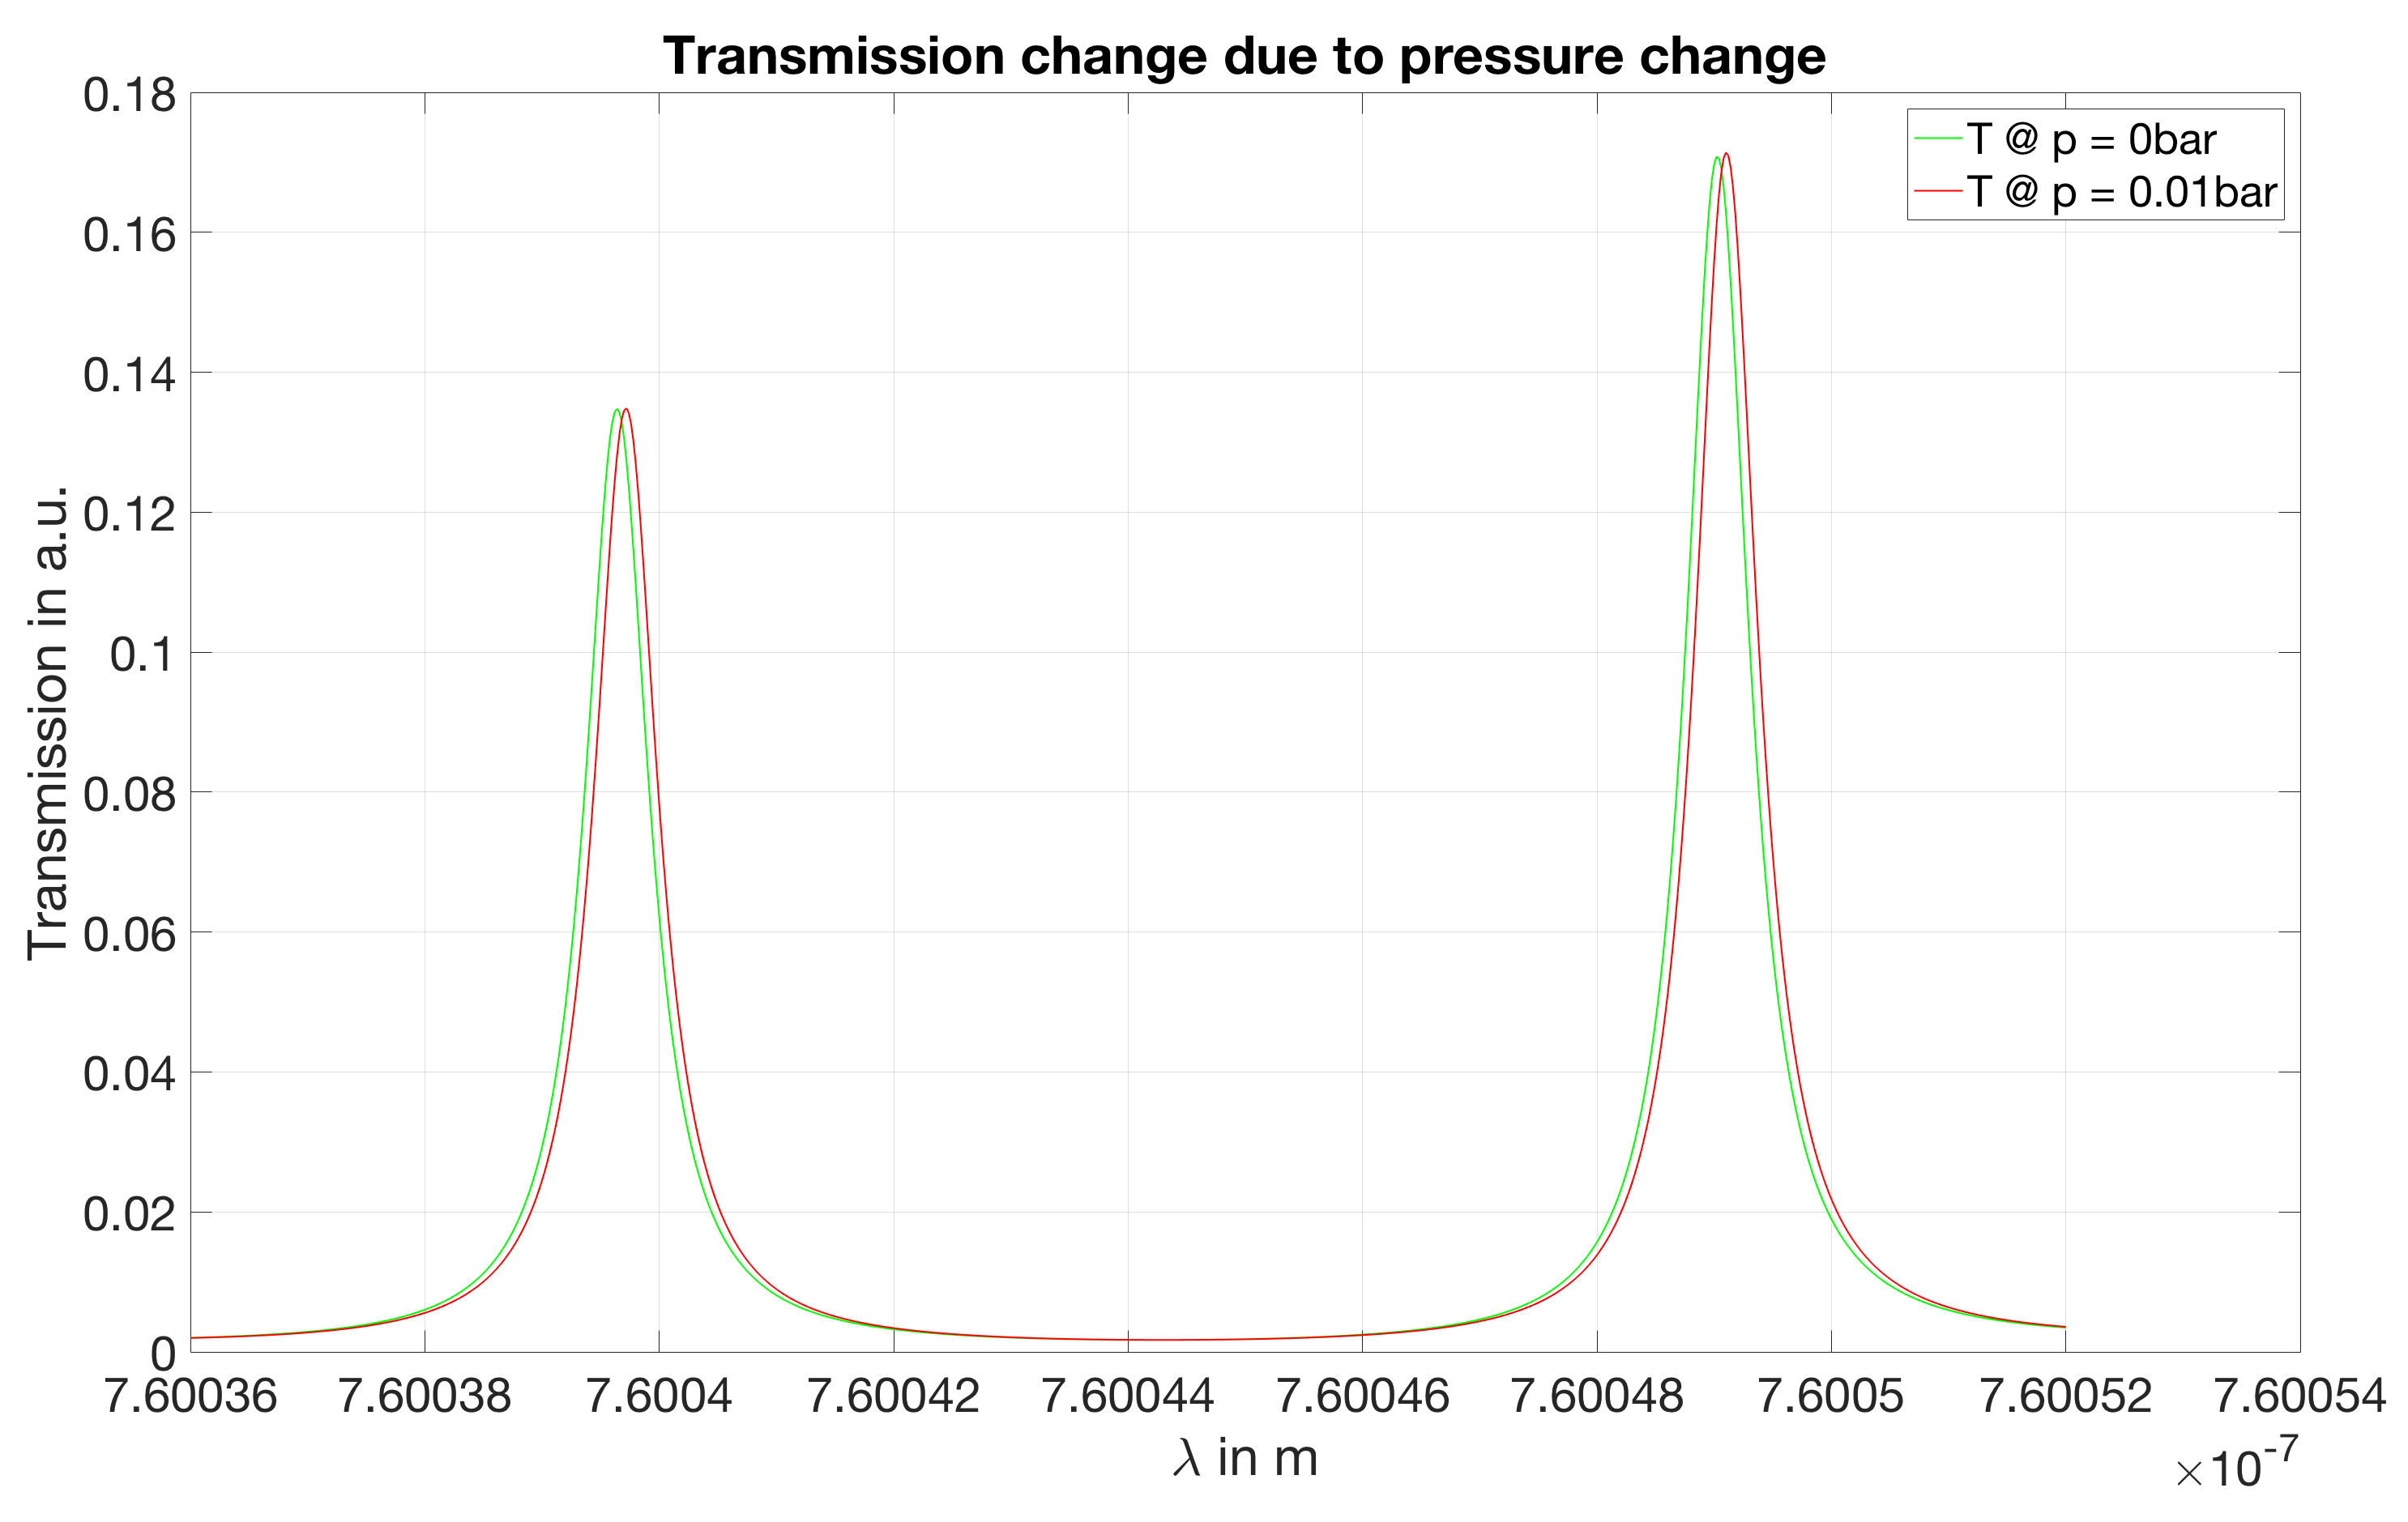
\includegraphics[width = \textwidth, height=0.3\textheight]{05_OUSD/images/transmissionChangePressure.png}
	\end{minipage}
	b)
	\begin{minipage}{0.5\textwidth}
		
		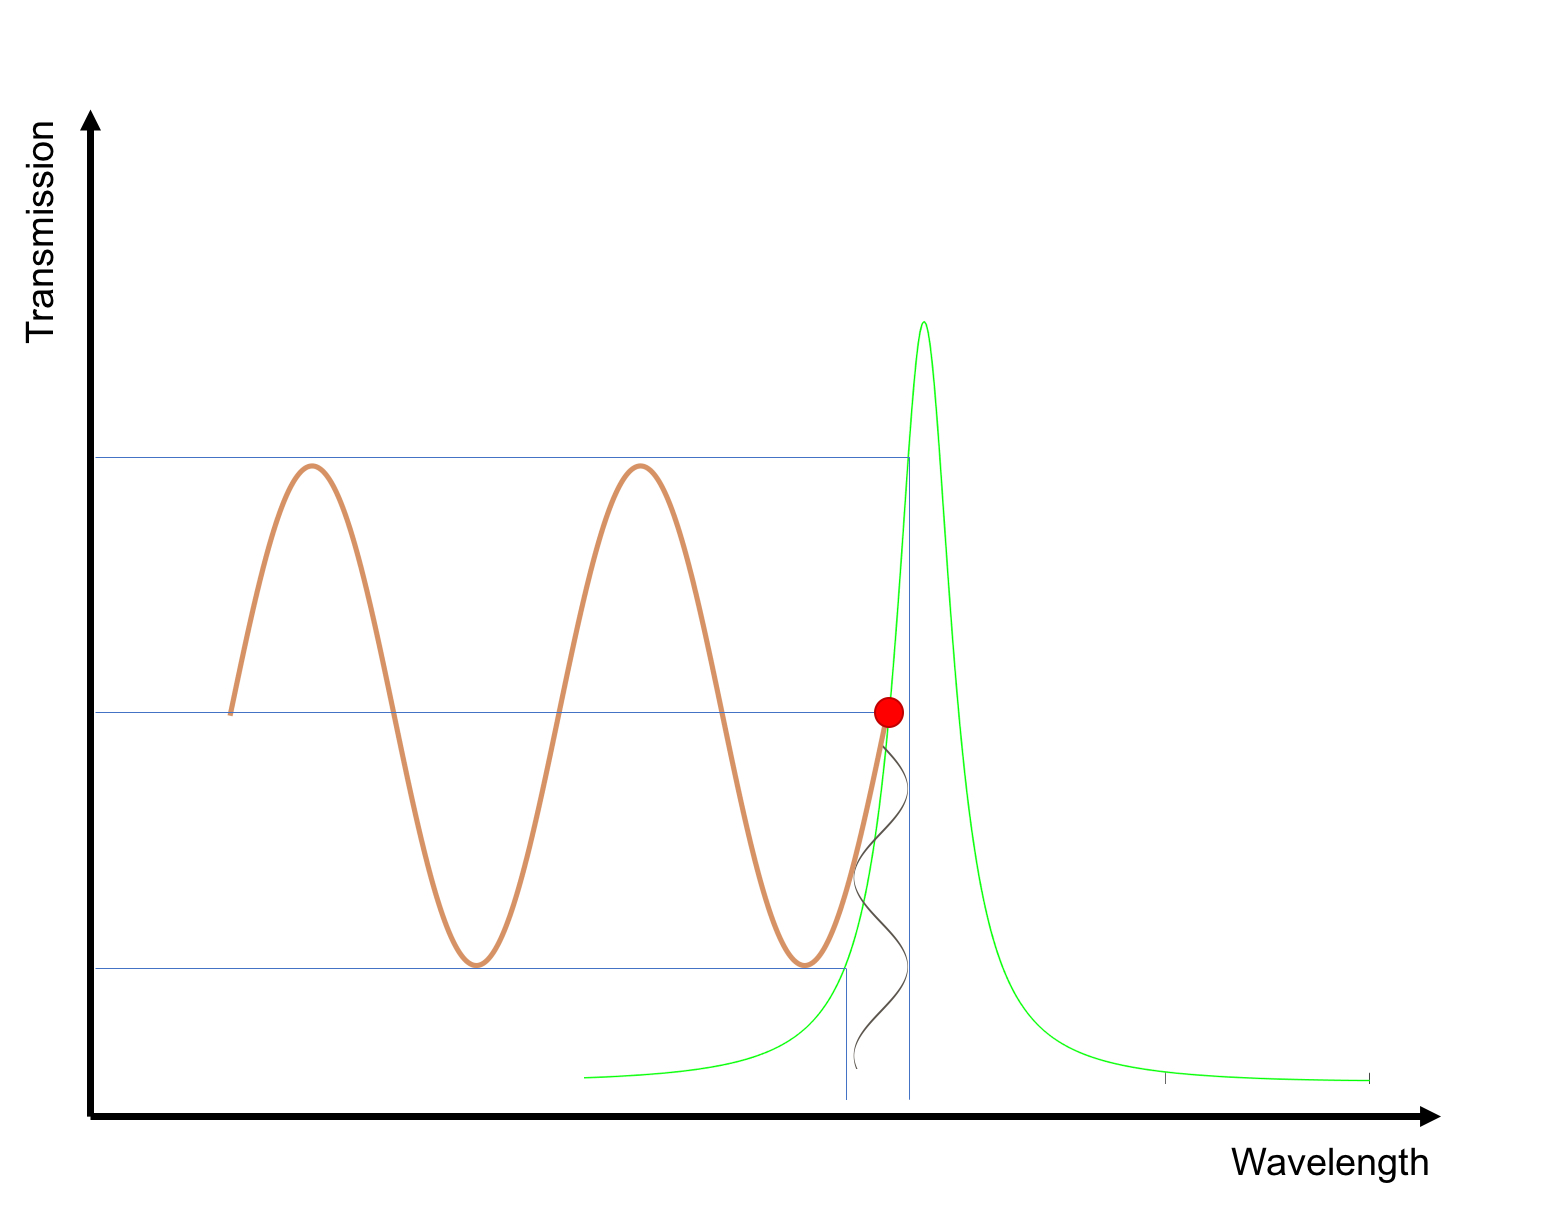
\includegraphics[width = \textwidth, height=0.35\textheight]{05_OUSD/images/sigSchematic.jpg}
	\end{minipage}
	
	\caption{a) shows how a pressure change influences the transmission condition of the resonator and in b) the response of the system to an incoming sinusoidal pressure wave is shown.}
	\label{fig:transmissionChange}
\end{figure}
 
Therefore figure \ref{fig:transmissionChange} a) shows a simulated transmission pattern at ambient pressure (green line) and at a constant pressure higher than the ambient pressure. The chosen pressure level is higher than a typical photoacoustic amplitude (red line), to better illustrate the effect. Thus, a shift towards longer wavelengths in the transmission pattern, can be seen. The simulation were done with water as a medium between the mirrors and its elasto-optic coupling coefficient $\frac{\mathrm{d}n}{\mathrm{d}p} = 1.35\; \mathrm{x} \;10^{-5} bar^{-1}$.\\
In figure \ref{fig:transmissionChange} b) the response to an incoming sinusoidal pressure change is shown. The system is regulated to hold its working point at a wavelength, there the transmission gradient (highlighted by the red point) has its maximum at ambient pressure. In order to keep this point stable the system is adjusted in a way that environmental stress is eliminated. But if a pressure wave in the $MHz$ range hits the resonator system the control is to slow to react and the red point moves as the transmission pattern moves, as shown in figure \ref{fig:transmissionChange} b). This leads to a change in the light intensity, which leaves the resonator. A photodetector that is placed behind the FPI converts the light into a voltage signal. 

\subsection{OUSD setup}

As shown in figure \ref{fig:FPIschematic} an induced ultrasonic wave travels back the optical path and interferes with the media between the two partially transmitting mirrors. The chosen medium were water, because its cheap and durable. The other feasibility would be FC77 an inert, dielectric liquid with higher $\frac{\mathrm{d}n}{\mathrm{d}p}$ than water, but because it volatilizes quickly, it is not suitable for longer measurements. 

\begin{figure}[H]
	\centering
	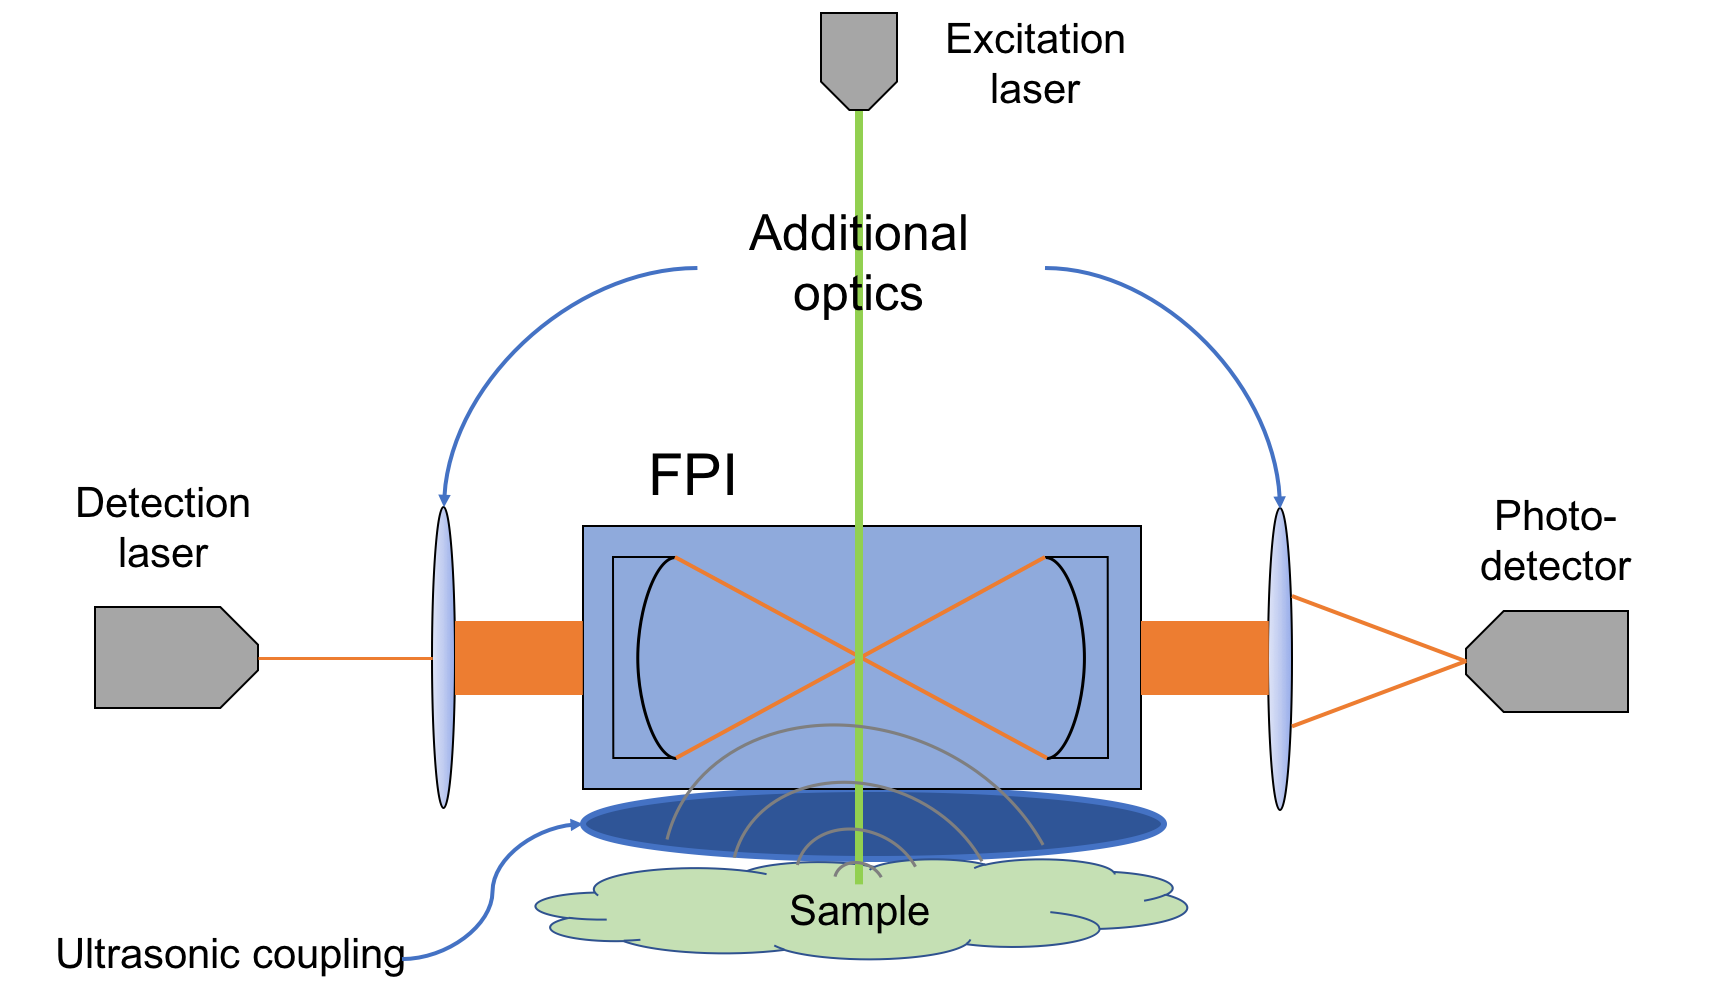
\includegraphics[height=0.4\textheight]{05_OUSD/images/FPIschematic.png}
	\caption{Schematic view of an optical ultrasonic detection system based on a Fabry–P\'{e}rot interferometer (FPI)}
	\label{fig:FPIschematic}
\end{figure} 

In order to make the system movable the detection laser and the excitation laser are brought to the system by optical fibers. The optics on the detection laser side consists of a bi-convex lens to collimate the beam and a plano-convex to focus it into the resonator. On the photodetector side a plano-convex lens focuses the transmitted light onto the photodiode. \\
The water of the resonator interior is restrained with the same transparent polymer membrane as in the OR-PAM setup.\\

\begin{figure}[H]
	a)
	\begin{minipage}{0.5\textwidth}
		
		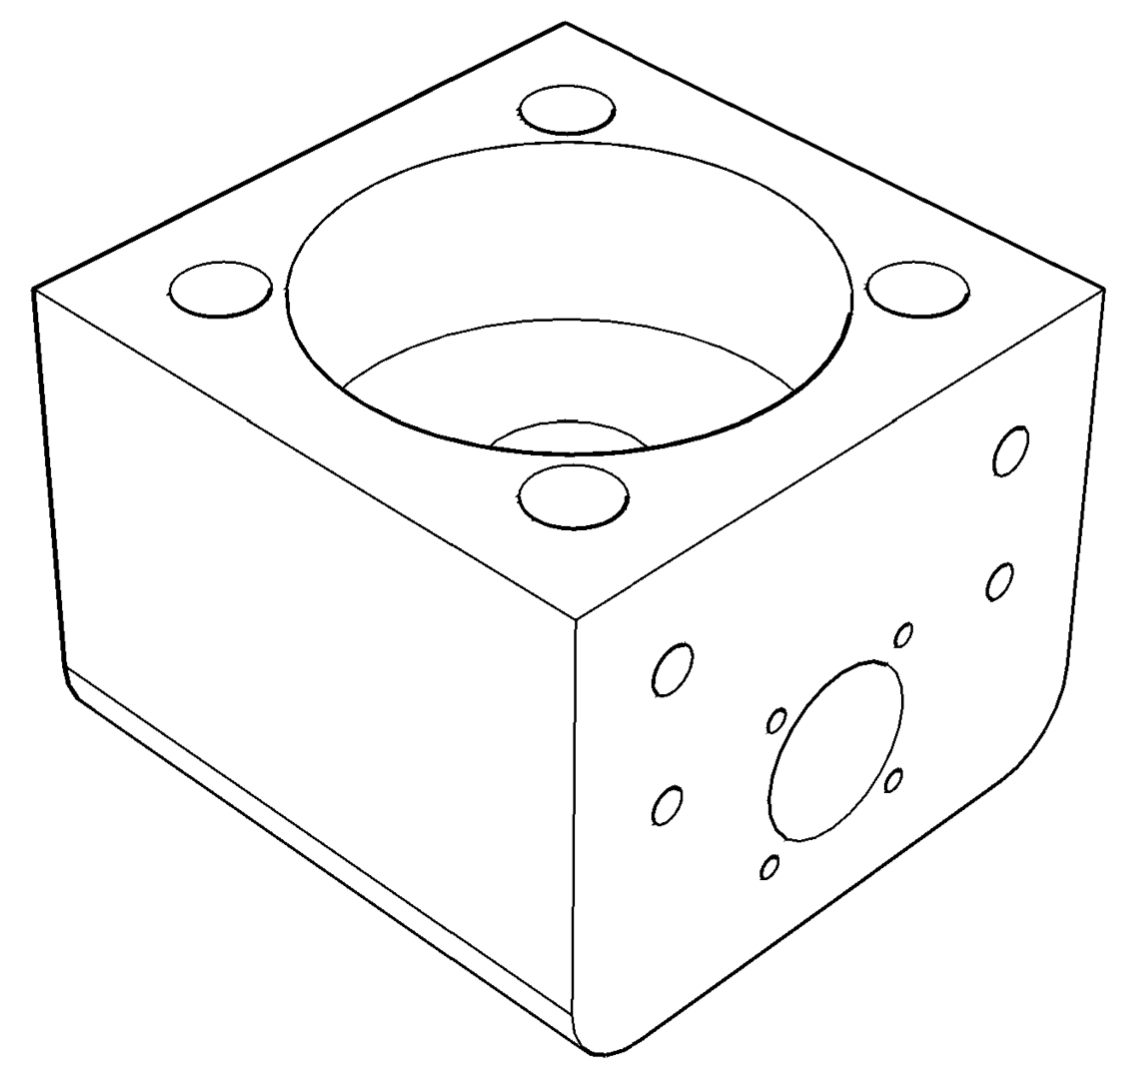
\includegraphics[width = \textwidth, height=0.35\textheight]{05_OUSD/images/res3D.jpg}
	\end{minipage}
	b)
	\begin{minipage}{0.5\textwidth}
		
		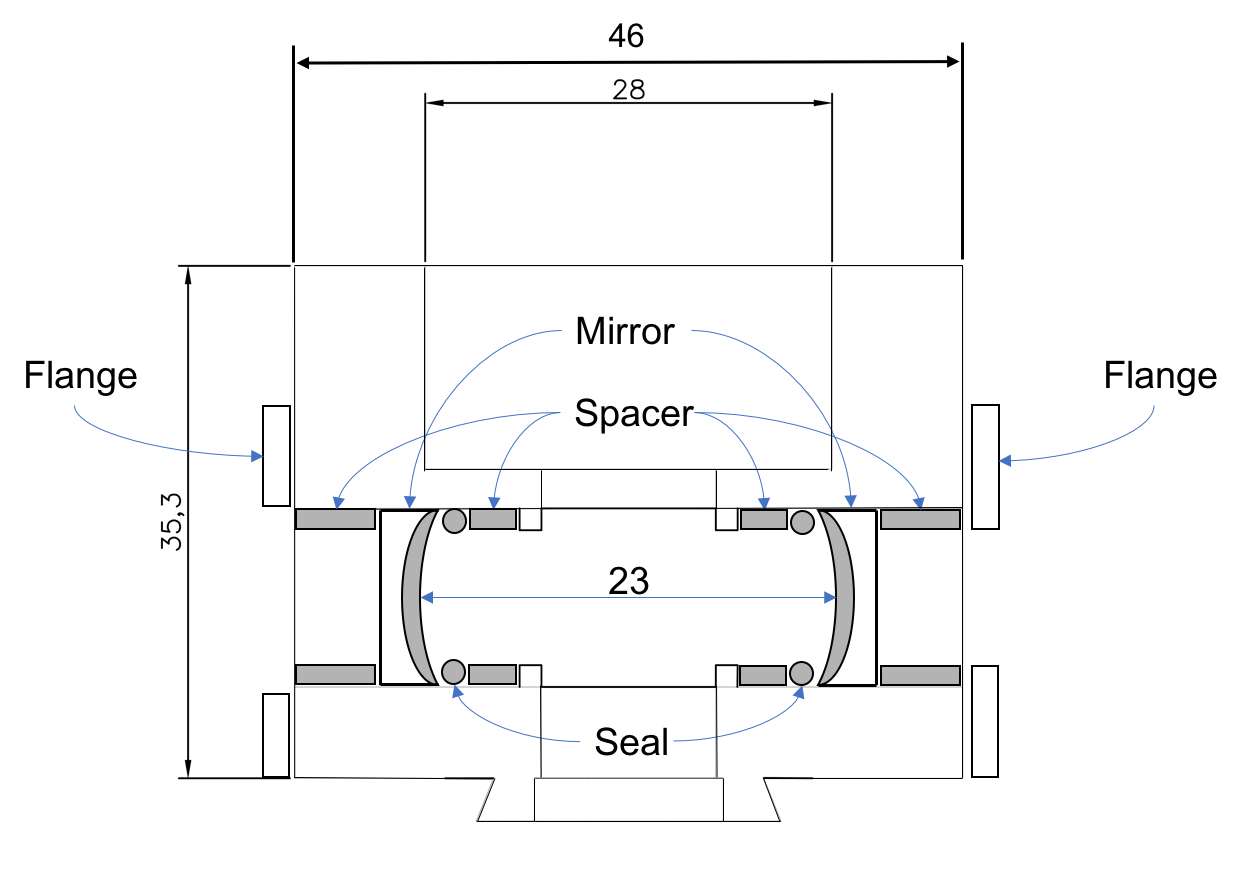
\includegraphics[width = \textwidth, height=0.3\textheight]{05_OUSD/images/resCut.jpg}
	\end{minipage}
	
	\caption{Schematic of the manufactured resonator. There a) shows a 3D model and b) a cut through it. All values are in $mm$.}
	\label{fig:resSchematic}
\end{figure}

Figure \ref{fig:resSchematic} b) shows a schematic cut through the resonator. The determination of the distance between mirrors gets discussed in section \ref{sec:resLength}. The flanges are pressing the mirrors against the spacers and seals to waterproof the system. Besides they are used to adjust the mirrors to match the focal points.\\
In figure Figure \ref{fig:resSchematic} a) a 3D model of the resonator is shown. The purpose of the holes in the front is to mount the flanges and the cage system. They also fix the cage system bars from the topside. There is also a hole on the topside to add an objective. \\

\subsection{System development}
\label{sec:sysDev}
This section shows the determination of the basic parameters of the resonator and mirrors. At first a resonator length is defined, followed by the simulation of the layer system that is coated onto the plane-concave lenses.\\
The system should be stable, but also have a maximum sensitivity for changes in the refractive index. Furthermore, the cutoff frequency should be as high as possible. 

\subsubsection{Resonator stability considerations}

There are several possibilities to setup a multi-beam interferometer, called resonator. For the specification of a stable system, a symmetrical ray profile and a minimum waist radius $w_0$. The waist radius can be written as

\begin{equation}
 w_0 = \left(\frac{\lambda L}{\pi}\right)^{1/2} \cdot \left(\frac{g_1 g_2(1-g_1g_2)}{(g_1 + g_2 - 2g_1g_2)^2}\right)^{1/4}
 \label{eq:w_0Res}
\end{equation}
\\
where $L$ is the resonator length, $\lambda$ the wavelength and $g_{1,2}$ are 

\begin{equation}
	g_{1,2} = 1-\frac{L}{R_{1,2}} 
	\label{eq:g1g2}
\end{equation}
\\
where $R_1$ and $R_2$ are the mirror radii \cite{eichler:laser}.  \\
Only configurations that meet the condition $0 \leq g_1 g_2 \leq 1$ are stable. Figure \ref{fig:resStability} shows all possible setups for a FPI. There only the blue shaded areas mark stable configurations.  

\begin{figure}[H]
	\centering
	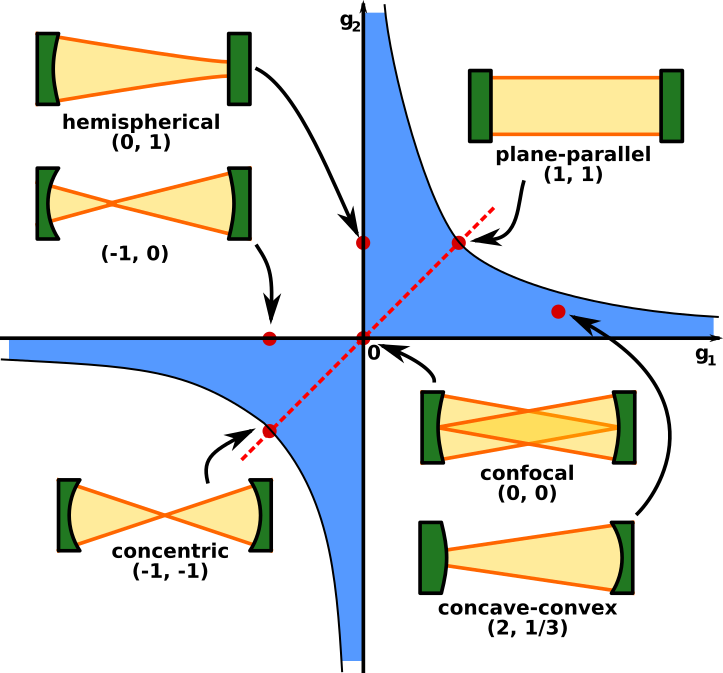
\includegraphics[height=0.4\textheight]{05_OUSD/images/Laser_resonator_stability.png}
	\caption{Resonator stability diagram for all possible arrangements of two mirrors. The blue shaded areas mark stable conditions, beyond them the system gets instable \cite{wiki:resStability}.}
	\label{fig:resStability}
\end{figure} 

In this case stable means that the light energy is located nearby the optical axis of the resonator and due to the finite mirror diameter, the diffraction losses are minimal. For unstable systems this means high diffraction losses \cite{eichler:laser}. 

\subsubsection{Resonator length determination}
\label{sec:resLength}
For the system, two plane concave mirrors from Edmund Optics (45016) with a diameter of 12~$mm$ and a radius of -12.40~$mm$, were chosen. Therefore the area of interest in figure \ref{fig:resStability} is the third quadrant. Thereby the mirrors are even so the red line marks all possible distance cases. The confocal case is the most stable one, but also with the least sensitivity. Vice versa the concentric case has the highest sensitivity, but is almost unstable.\\
Due to this conditions $g_1$ is equal $g_2$ and the formula for $w_0$ reduces to 

\begin{equation}
w_0 = \sqrt{\frac{\lambda}{2 \pi} \sqrt{L(2R-L)}}
\label{eq:w_0Reduced}
\end{equation}
\\
Figure \ref{fig:resLength} shows a simulation for the given mirror values. Also the wavelength were set to 760~$nm$, as this is the center frequency of the used tunable laser TEC 500 from Sacher Lasertechnik.

\begin{figure}[H]
	\centering
	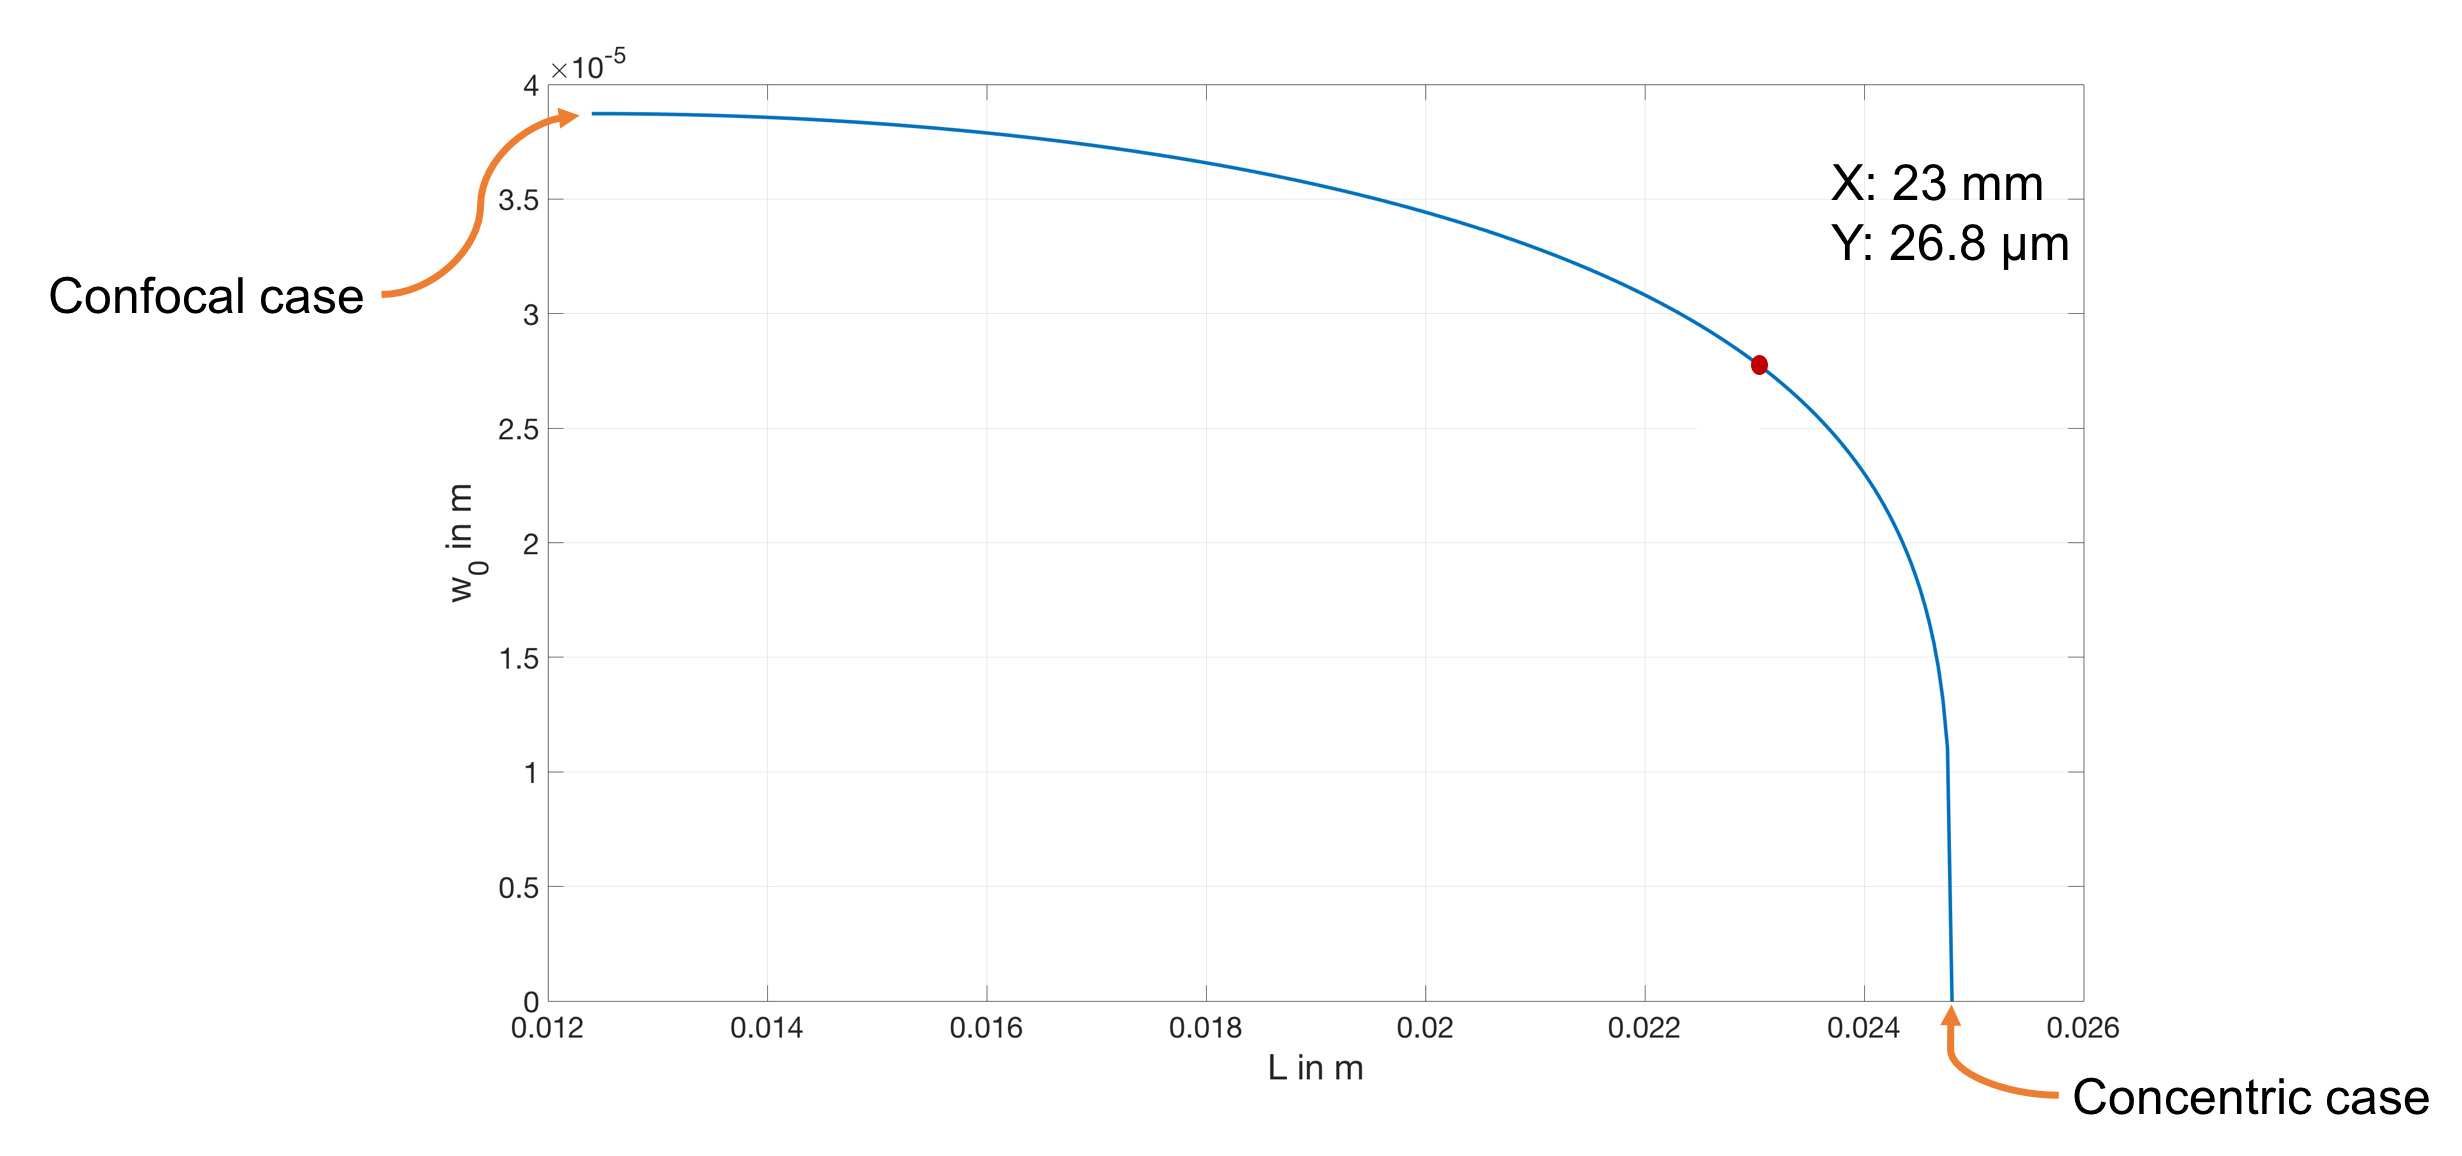
\includegraphics[ height=0.35\textheight]{05_OUSD/images/resLength.png}
	\caption{Waist radius in relation to the distance between the mirrors.}
	\label{fig:resLength}
\end{figure} 

The chosen distance between the mirrors were 23~$mm$. The red dot marks this point in Figure \ref{fig:resLength}. This value is as close to the confocal case as necessary, but distant enough to the concentric case to avoid instability, therefore the waistradius is 26.8~$\mu m$. 

\subsubsection{Mirror coating material considerations}

In order to find a suitable coating material and technique for the mirrors, some considerations have to be done. Primer terms are, that they can be coated at the institute and that the coating is durable against corrosion due to the alternating contact with water and air.\\
Therefore the physical vapor deposition (PVD) unit at the facility is chosen. In PVD a small cup, containing the selected metal, inside an evacuated chamber gets heated up to its evaporation temperature. The vaporized material spreads, due to its thermal energy, towards the target. The coating thickness is controlled by the exposure time of the target. Figure \ref{fig:CoatingMat} shows the spectral reflectivity, over a wavelength range from 200~$nm$ to 1200~$nm$, of materials that are eligible. 
 
\begin{figure}[H]
	\centering
	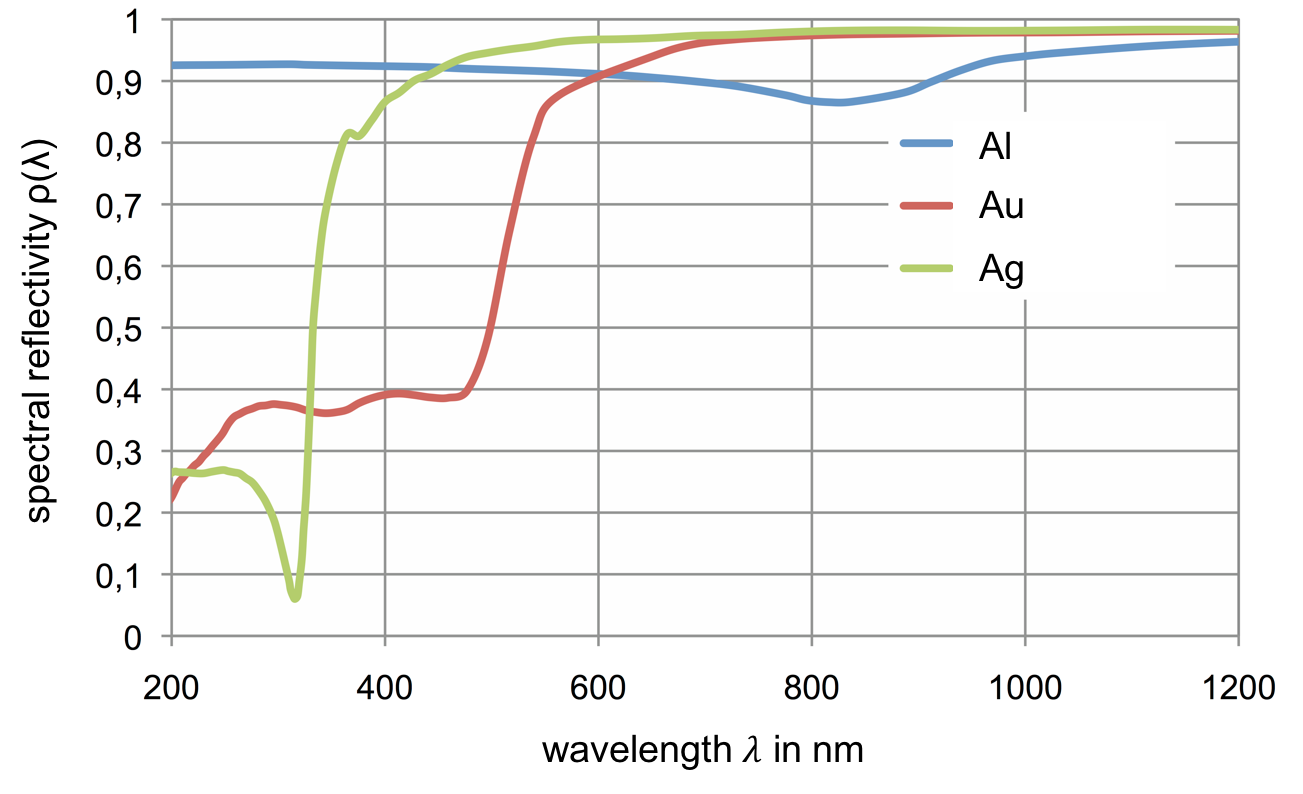
\includegraphics[width = 0.75\textwidth, height=0.3\textheight]{05_OUSD/images/coatingMat.png}
	\caption{Spectral reflectivity $\rho$ in dependence of the wavelength $\lambda$ for aluminum (Al), gold (Au) and silver (Ag).  \cite{bauelOptik}}
	\label{fig:CoatingMat}
\end{figure}

The chosen material should have a high reflectivity around 760~$nm$ and to be corrosion resistant. As gold has nearly the same reflectivity as silver at the desired wavelength, but a much higher durability, the chosen material for the mirror coating is gold. 

\subsubsection{Transfer matrix method (TMM)}

The calculation of an optical multilayer system can be done with the Transfer matrix Method. Especially the transmission and reflection of an optical multilayer system are of particular interest, to determine the the thickness of the gold layer. \\
Here the assumption is done that an incident beam is s-polarized and perpendicular to the plane. Besides that the layers are plain and expand infinite in z-direction. 
The Fresnel-coefficients are then given by

\begin{equation}
r_{ij} = \frac{n_i - n_j}{n_i + n_j};\; t_{ij} = \frac{2 \cdot n_i}{n_i + n_j}
\label{eq:r&t}
\end{equation}
\\
There $n$ is the complex refractive index $n = \tilde{n} + i \kappa$ that contains $\tilde{n}$, the refractive index and $\kappa$, the extinction coefficient. Furthermore, i is the current and j the following layer. 

\begin{figure}[ht]
	\centering
	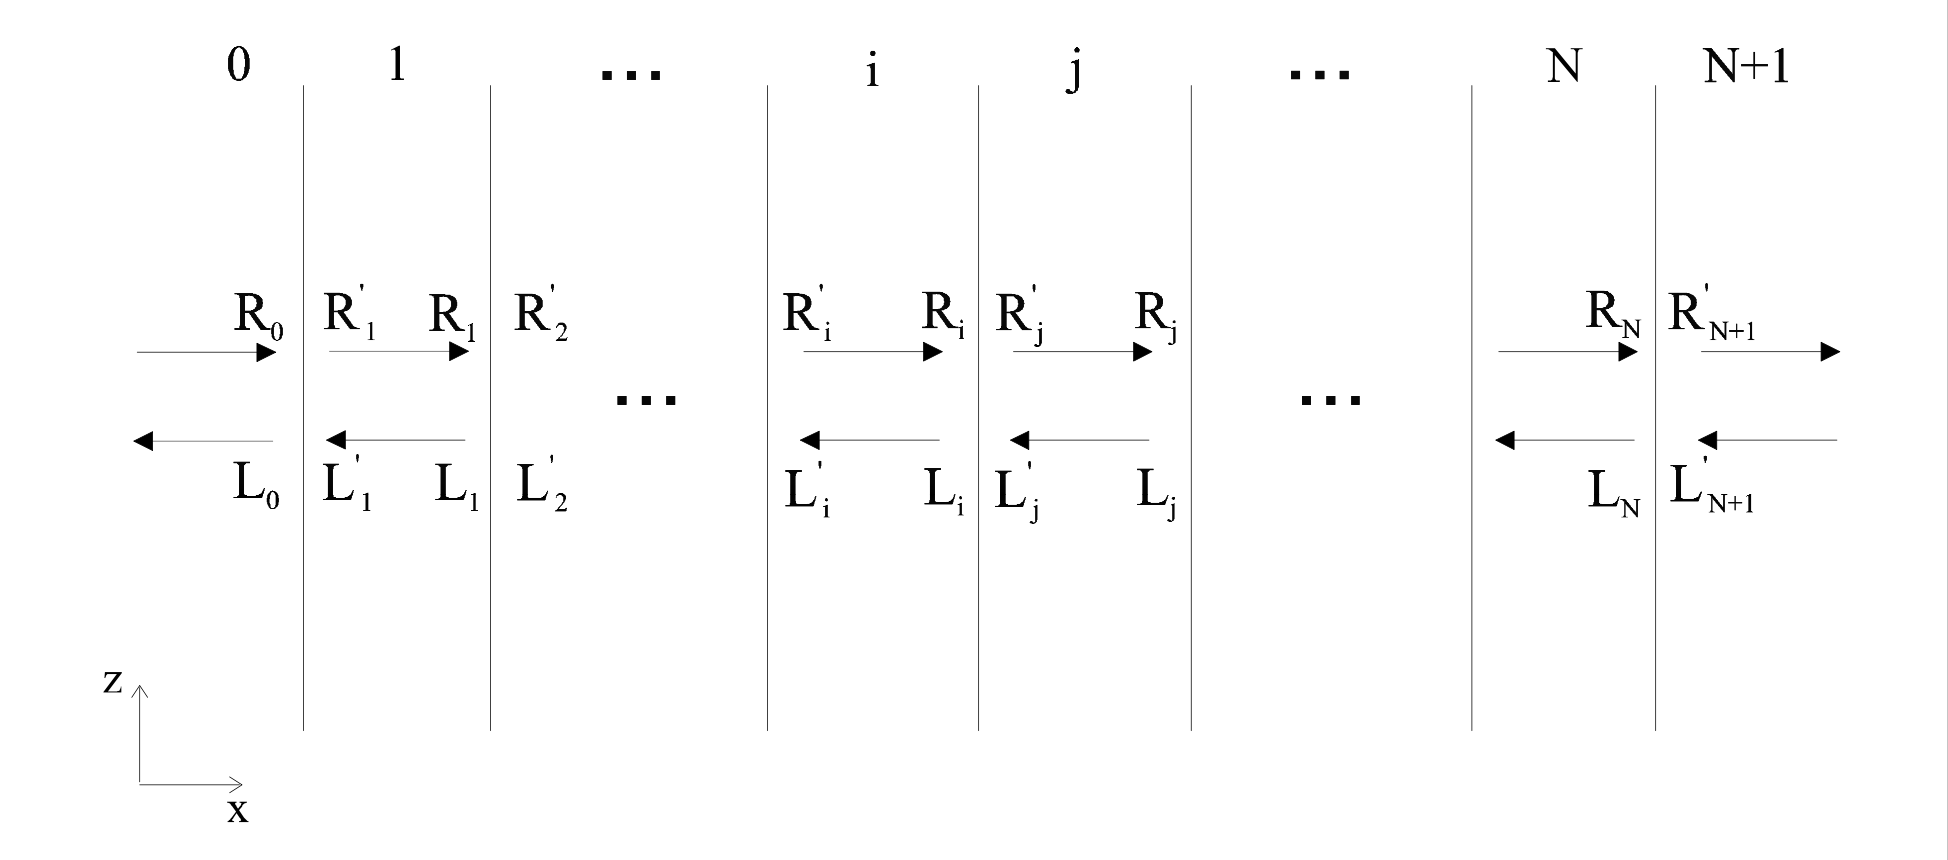
\includegraphics[width = 0.9\textwidth]{05_OUSD/images/SchemaSchichtsystem.png}
	\caption[Schematic of a layersystem]{Schematic view of a layer system \cite{Podgorsek:Vielfachschichten}}
	\label{fig:schemlayer}
\end{figure}

Figure \ref{fig:schemlayer} schematically shows the principle of a layer system. Every section contains a combination of left and right moving plane wave components. This sums up to a solution for the electrical field given by

\begin{equation}
E_i(x) = R_i\;exp(ik_{xi}x) + L_i\;exp(-ik_{xi}x) 
\label{eq:E_i}
\end{equation}
\\
where $ R_i $ is the ratio that goes in positive and $L_i$ in negative x-direction. \\
The left side of the boundary is defined by $ \begin{pmatrix}R_i \\ L_i\end{pmatrix} $  and $ \begin{pmatrix}R_j' \\ L_j'\end{pmatrix}  $ to the right. Based on the continuity condition, the amplitude vectors on both sides of the interface can be combined. 

\begin{equation}
\begin{pmatrix}R_i \\ L_i\end{pmatrix}  = \frac{1}{t_{ij}} \cdot 
\begin{bmatrix}
1 & r_{ij} \\ r_{ij} & 1
\end{bmatrix}  \begin{pmatrix}R_j' \\ L_j'\end{pmatrix}  = D_{ij} \begin{pmatrix}R_j' \\ L_j'\end{pmatrix} 
\label{eq:DMat}
\end{equation}
\\
$D_{ij}$ is the transfer matrix that describes the transition from layer $i$ to $j$. Inside a layer the vectors differ in a passing phase $\phi_i$.

\begin{equation}
\phi_i = k_0 \cdot n_i \cdot d_i
\label{eq:matKoeff}
\end{equation}
\\
Where $k_0$ is the incident wave vector, $n_i$ the complex refractive index of the current layer and $d_i$ the layer thickness. This phase is described by a phase matrix $P_i$

\begin{equation}
\begin{pmatrix}R_i' \\ L_i'\end{pmatrix}= 
\begin{bmatrix}
\exp(j \cdot \Phi_i) & 0 \\ 0 & \exp(-j \cdot \Phi_i)
\end{bmatrix}\begin{pmatrix}R_i \\ L_i\end{pmatrix}
= P_i \begin{pmatrix}R_i \\ L_i\end{pmatrix}
\label{eq:PMat}
\end{equation}
\\
This follows:
\begin{equation}
\begin{pmatrix}R_i' \\ L_i'\end{pmatrix}= 
P_i\;D_{ij} \begin{pmatrix}R_j' \\ L_j'\end{pmatrix}
\end{equation}
\\
Next a total transfer matrix $M$ is defined. It consists the product of all transfer($D$) and phase($P$) matrices to describe a layer system of $N$ layers

\begin{equation}
\begin{pmatrix}R_0 \\ L_0\end{pmatrix}
= M \;  \begin{pmatrix}R_{N+1}' \\ L_{N+1}' \end{pmatrix}
\label{eq:v0linkTovN+1}
\end{equation}

\begin{equation}
M = \begin{bmatrix}
M_{11} & M_{12} \\ M_{21} & M_{22}
\end{bmatrix} 
= D_{01} \cdot \prod \limits_{i=1}^{N} P_i \; D_{i, i + 1} 
\label{eq:matTMM}
\end{equation}
\\
By means of M, it is possible to calculate R and T. In order to do so, a wave hitting the layer system with amplitude $R_0$ and $L_{N+1}' = 0$, as shown in Figure \ref{fig:schemlayer}, can be supposed. Due to that, equation \eqref{eq:v0linkTovN+1} can be written as

\begin{equation}
R_0 = M_{11} \cdot R_{N+1}' \; ; \; L_0 = M_{21} \cdot R_{N+1}'
\end{equation}
\\
Therefore, the reflection and transmission coefficient are given by

\begin{equation}
r = \frac{L_0}{R_0} = \frac{M_{21}}{M_{11}} \; ; \;
t = \frac{R_{N+1}'}{R_0} = \frac{1}{M_{11}} 
\label{eq:rtCoef}
\end{equation}
\\
Finally R and T are determined:

\begin{equation}
R = \left\lvert \frac{M_{21}}{M_{11}}\right\rvert^2 \; ; \;
T = \left\lvert \frac{1}{M_{11}}\right\rvert^2
\label{eq:RT}
\end{equation}
\\
Therefore R and T depend on the wavelength, thickness of the layer and the complex reflection index that contains the extinction coefficient \cite{Podgorsek:Vielfachschichten}.

\subsubsection{Coating thickness determination with TMM}

In order to manufacture partially transmitting mirrors that fit into the system, a simulation were done with the help of the TMM. In figure \ref{fig:TMMsimLayersystem} the involved materials and their arrangement are shown . 

\begin{figure}[H]
	\centering
	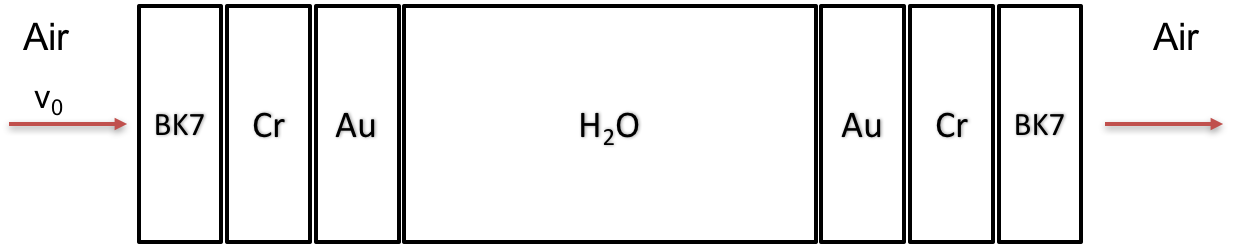
\includegraphics[height=0.15\textheight,width=\textwidth]{05_OUSD/images/TMM_schematisch.png}
	\caption{Schematic view of simulated layer system. The gold layer is variable, the others are fixed. For BK7 = 3.5~$mm$, Cr = 2~$nm$ and for H$_2$O = 23~$mm$.}
	\label{fig:TMMsimLayersystem}
\end{figure} 

The first layer is an air layer where the incident beam hits the system. Next one is the BK7 glass lens blank where the metals are coated onto. As those are concave, their waist thickness were taken. The chrome layer acts as an adherence layer for the following gold layer, but it barely affects the properties of the mirrors, due to the thickness of just a few atom layers. The H$_2$O layer has the thickness that was determined before in section \ref{sec:resLength}. At the end the vise versa configuration of the first mirror were established. The values for the complex refractive indexes are taken from the refractive index database \cite{rii}. The layer system from figure \ref{fig:TMMsimLayersystem}, were simulated in figure \ref{fig:transmission3D}, for a gold layer thickness range of 5~$nm$ to 70~$nm$.

\begin{figure}[H]
	\centering
	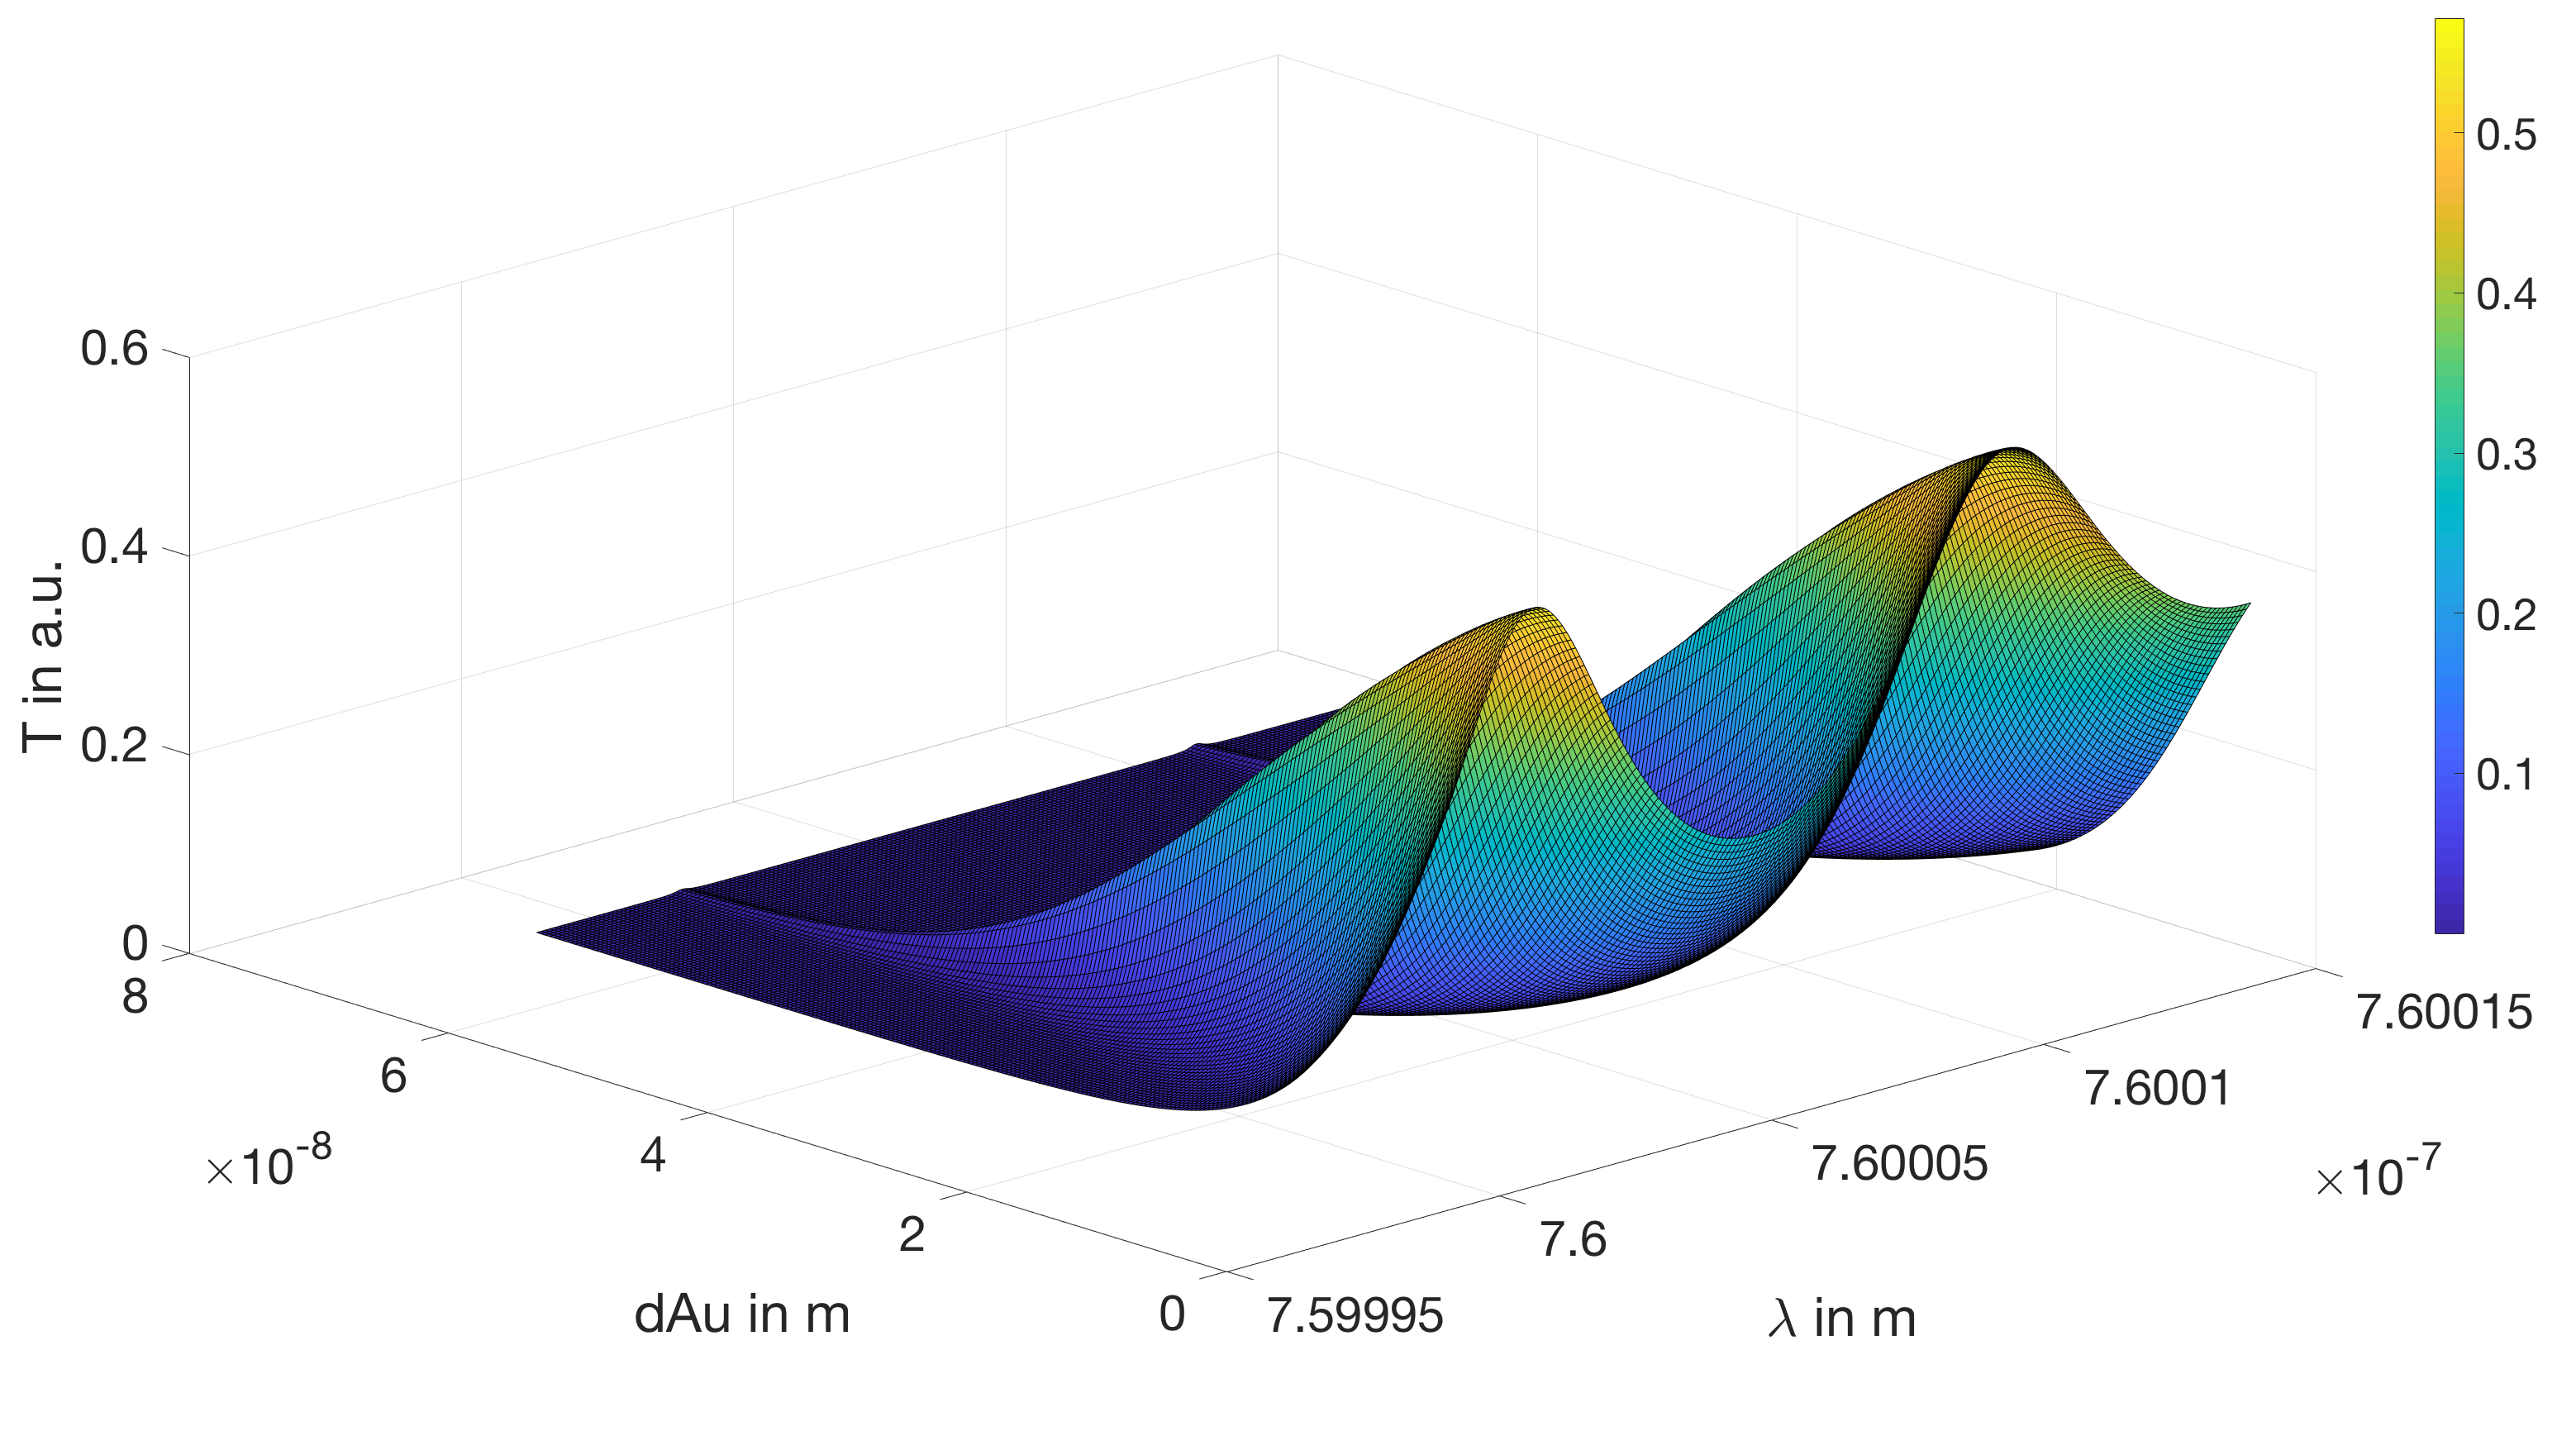
\includegraphics[height=0.47\textheight,width=\textwidth]{05_OUSD/images/transmission3D.png}
	\caption{Transmission pattern around the center frequency of the tunable laser in dependence of the gold layer thickness. The heatmap shows the transmission axis T in terms of color. The simulation were done with 200 points.}
	\label{fig:transmission3D}
\end{figure} 

As it can be seen, with increasing thickness of the gold layer, the transmission value decreases. For ultrasound detection the important value is the edge steepness of the transmission peaks. Figure \ref{fig:transDerivative} shows the maximum steepness values $\frac{\mathrm{d}T}{\mathrm{d}\lambda}$ dependent on the thickness of the gold layers.

\begin{figure}[H]
	\centering
	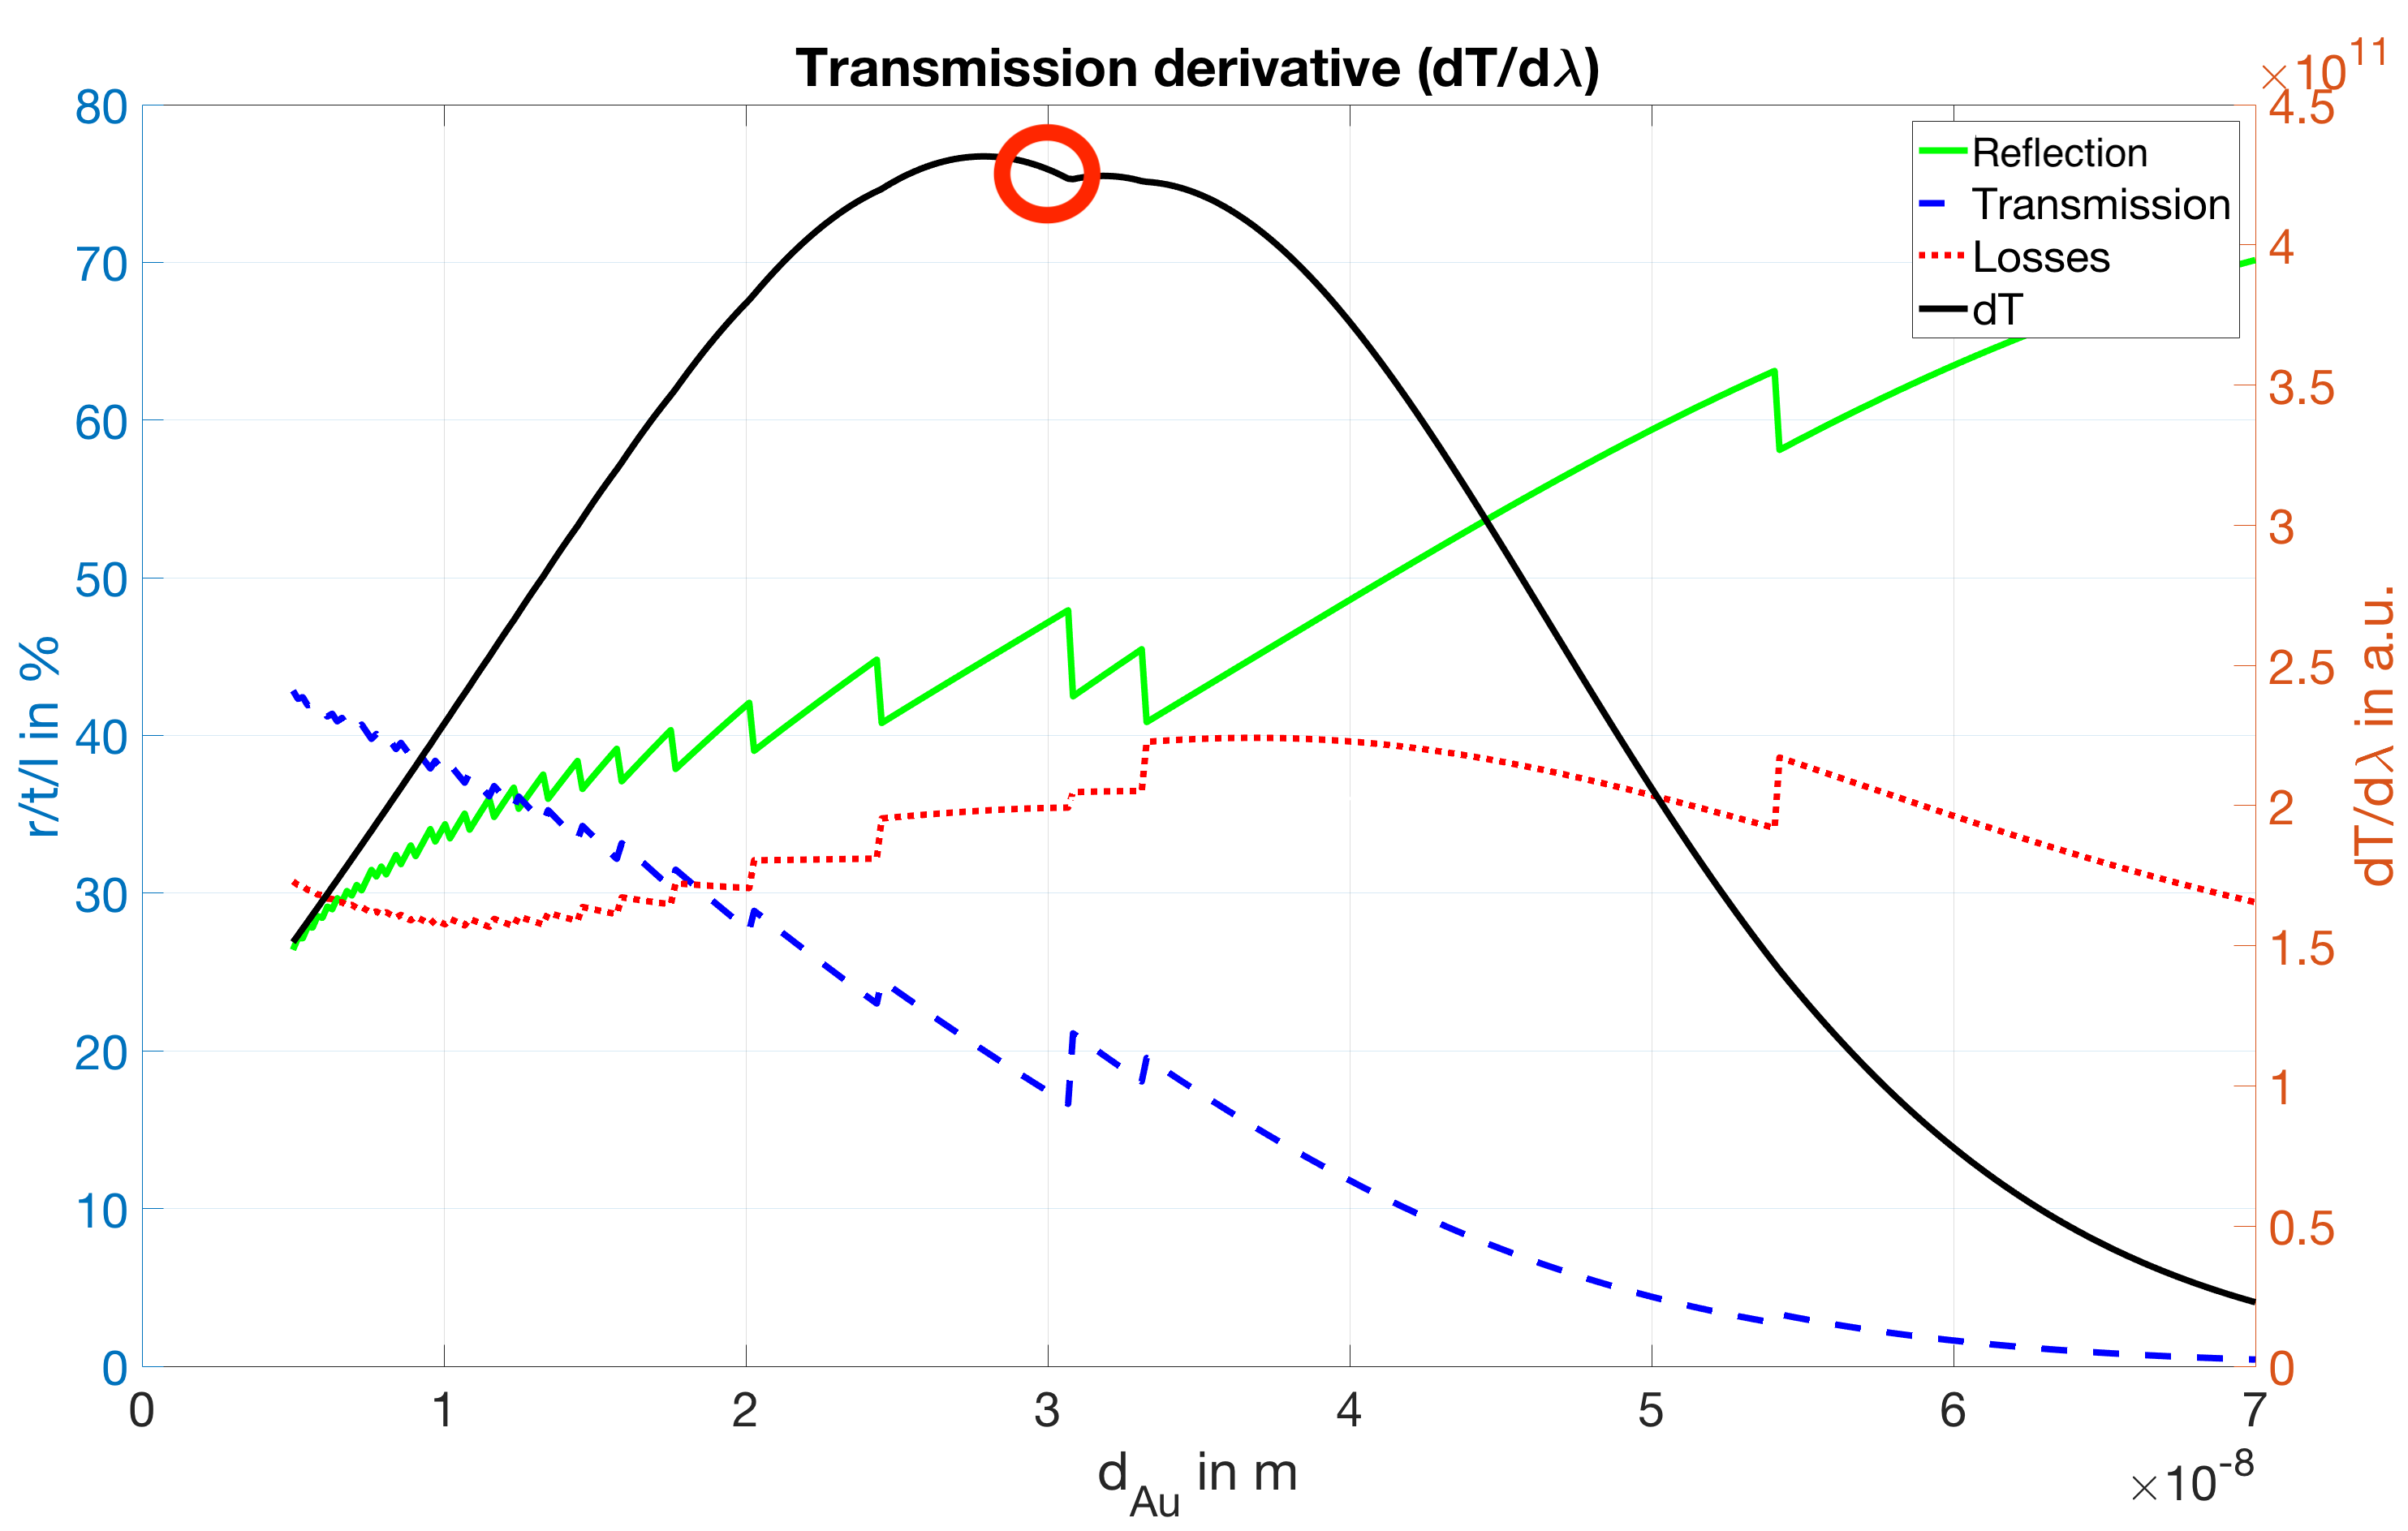
\includegraphics[height=0.56\textheight,width=1.1\textwidth]{05_OUSD/images/transDerivative.png}
	\caption{The black line shows the maximum values for the derivative of the transmission at a specific thickness of the gold layer and its corresponding axis is the right one. The values for transmission, reflection and losses are calculated based on this data. Besides the corresponding axis is the left one. The simulation were done with 200 points.}
	\label{fig:transDerivative}
\end{figure} 

The jumps in the lines for transmission, reflection and losses are a result of the varying points of maximum steepness. As there are two transmission peaks are considered in figure \ref{fig:transmission3D}, the maximum can either be at the first or second peak.\\
The maximum for $\frac{\mathrm{d}T}{\mathrm{d}\lambda}$, in figure \ref{fig:transDerivative}, is at about 30~$nm$ (red circle), therefore the mirrors were coated with this thickness value.  

\subsection{Cutoff frequency estimation}
\label{sec:cutOffFreq}

In order to estimate the cutoff frequency of the system, it can be assumed, that the light intensity in the middle of the resonator is rectangular distributed, as an approach to a Gaussian distribution, as illustrated in figure \ref{fig:lightDist} b). Therefore the width $d$ correspond to the FWHM of the cross section.  

\begin{figure}[H]
	\centering
	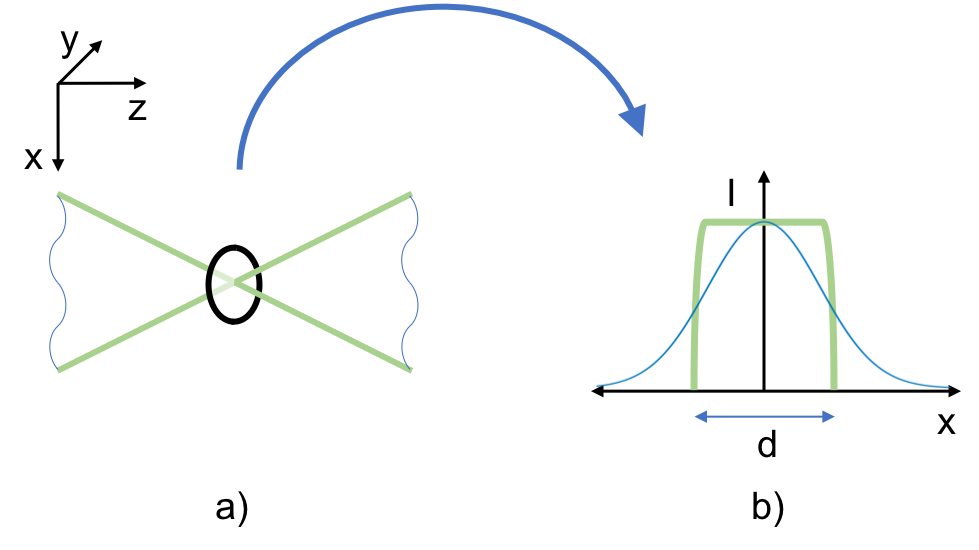
\includegraphics[height=0.4\textheight]{05_OUSD/images/lightDistribution.png}
	\caption{In a) the intersect of the mirror focuses is shown. The investigated cross section is marked. Furthermore, the origin lies in the center of the circle in a) and b) shows the supposed light distribution.}
	\label{fig:lightDist}
\end{figure} 

This allows us to simplify the calculation. The shortest incoming pressure wave has to have a wavelength of $\lambda/2$ because the change of the refractive index, whether the amplitude is positive or negative, is directed in one direction. For example, a full wavelength would cancel out the change of the refractive index because of the positive and negative amplitude. Therefore $\lambda$ has to be $\lambda_{cutoff} = 2 \cdot d$. This follows the equation

\begin{equation}
f_{cutoff} = \frac{c_{H_2O}}{\lambda_{cutoff}} =\frac{c_{H_2O}}{4 \cdot w_0}
\label{eq:fCutoff}
\end{equation}
\\
where $c_{H_2O}$ is the speed of sound in water at a given temperature and $w_0$ is the calculated waist radius. With the values for $c_{H_2O}$ = 1483.2~$m/s$ at 20~$^\circ C$ \cite{Haynes:physicalProperties} and as calculated in for in section \ref{sec:resLength}, $w_0$ = 26.8~$\mu m$, the cutoff frequency becomes $f_{cutoff}$ = 13.8~$MHz$. The actual value may be at a higher frequency due to the Gaussian beam profile. 

\subsection{Measuring-methods to determine the ultrasonic pressure}
\label{sec:pMeasureMeth}
In order to get an idea about the pressure amplitude range of the ultrasonic transducers that were used to determine the transfer function, two measurement setups were built. The first method were a needle hydrophone, there the ultrasonic field gets detected punctual and the second one is based on a Mach-Zehnder interferometer. Where the pressure amplitude is integrated over a line just like the OUSD system does. 
 
\subsubsection{Needle hydrophone}

A needle hydrophone is a PVDF foil which is glued on top of a metal tube. For this setup the Müller-Platte Nadelsonde from Dr. Müller Instruments were used, there the tip has a cross section of 1.2~$mm$. Figure \ref{fig:needleHydrophone} shows the measurement setup. 

\begin{figure}[H]
	\centering
	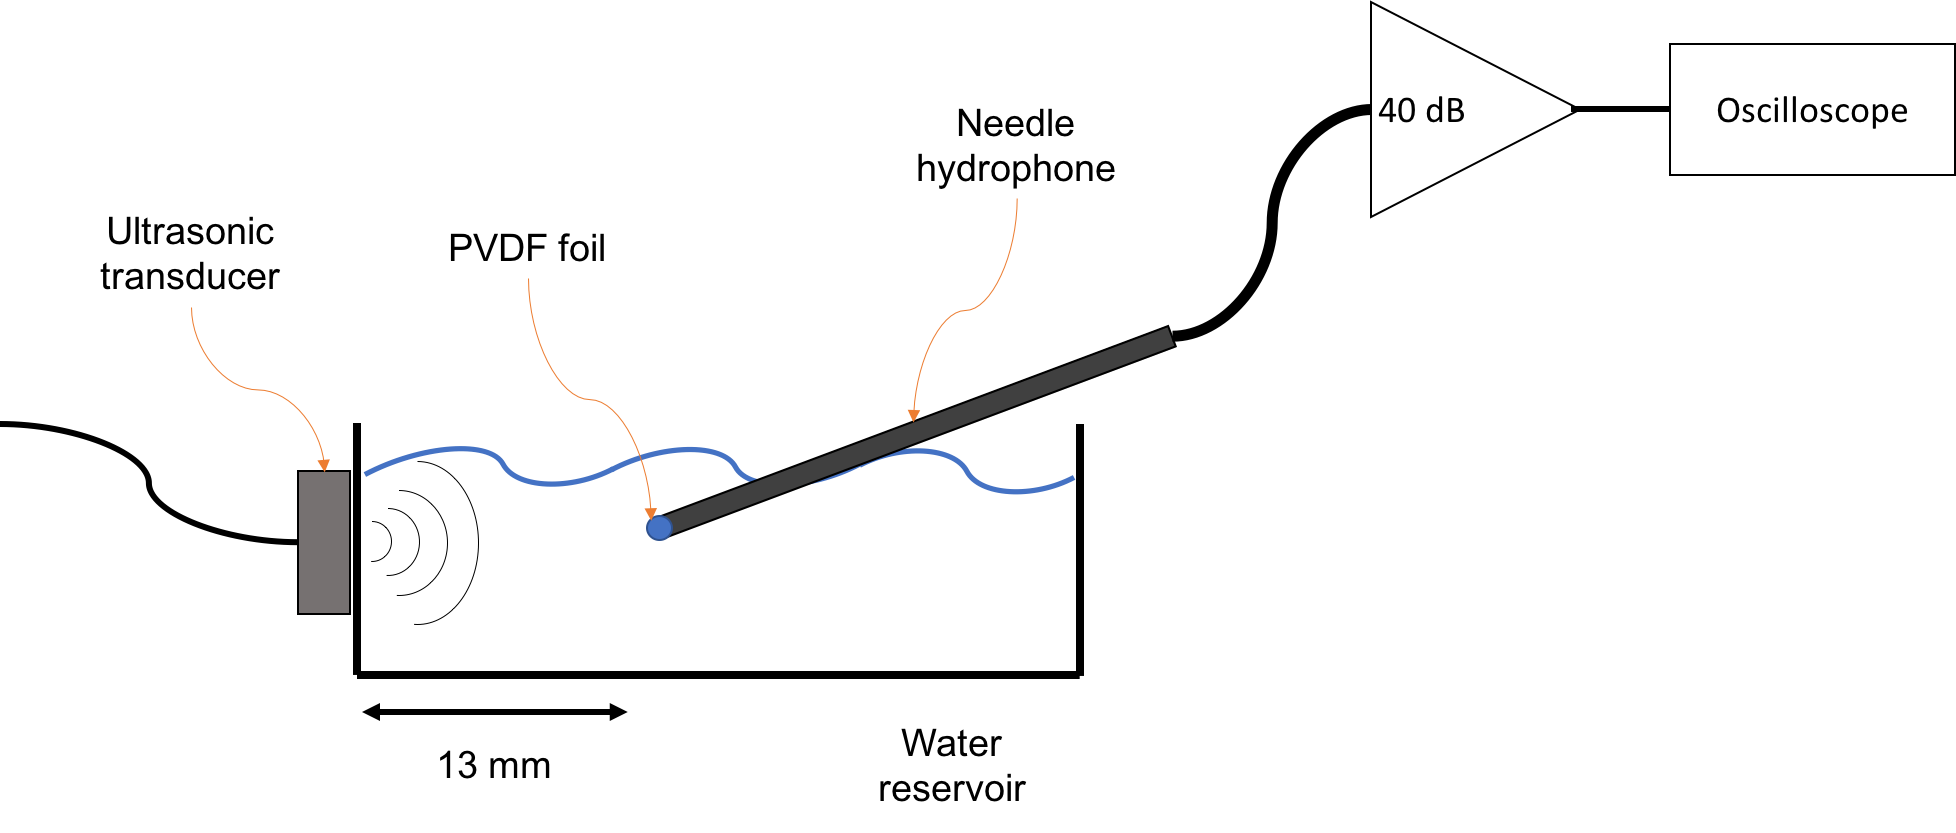
\includegraphics[width = \textwidth, height=0.3\textheight]{05_OUSD/images/NeedleHydro.png}
	\caption{Schematic of a needle hydrophone setup.}
	\label{fig:needleHydrophone}
\end{figure} 

The ultrasonic transducer were acoustically coupled onto the water reservoir, there the needle hydrophone were placed 13~$mm$ away from the transducer. This is about the working distance between the sample and the optical path of the detection laser in the OUSD system. \\
The ultrasonic wave that were detected gets amplified and displayed by an oscilloscope. With a conversion relation (here the sensitivity is 1.3~$\frac{mV}{bar}$) the voltage signal were translated into a pressure signal.  


\subsubsection{Mach-Zehnder interferometer}

In order to verify the results of the needle hydrophone a Mach-Zehnder interferometer were built. Figure \ref{fig:MZinterSchem} shows the schematic measurement setup.  

\begin{figure}[H]
	\centering
	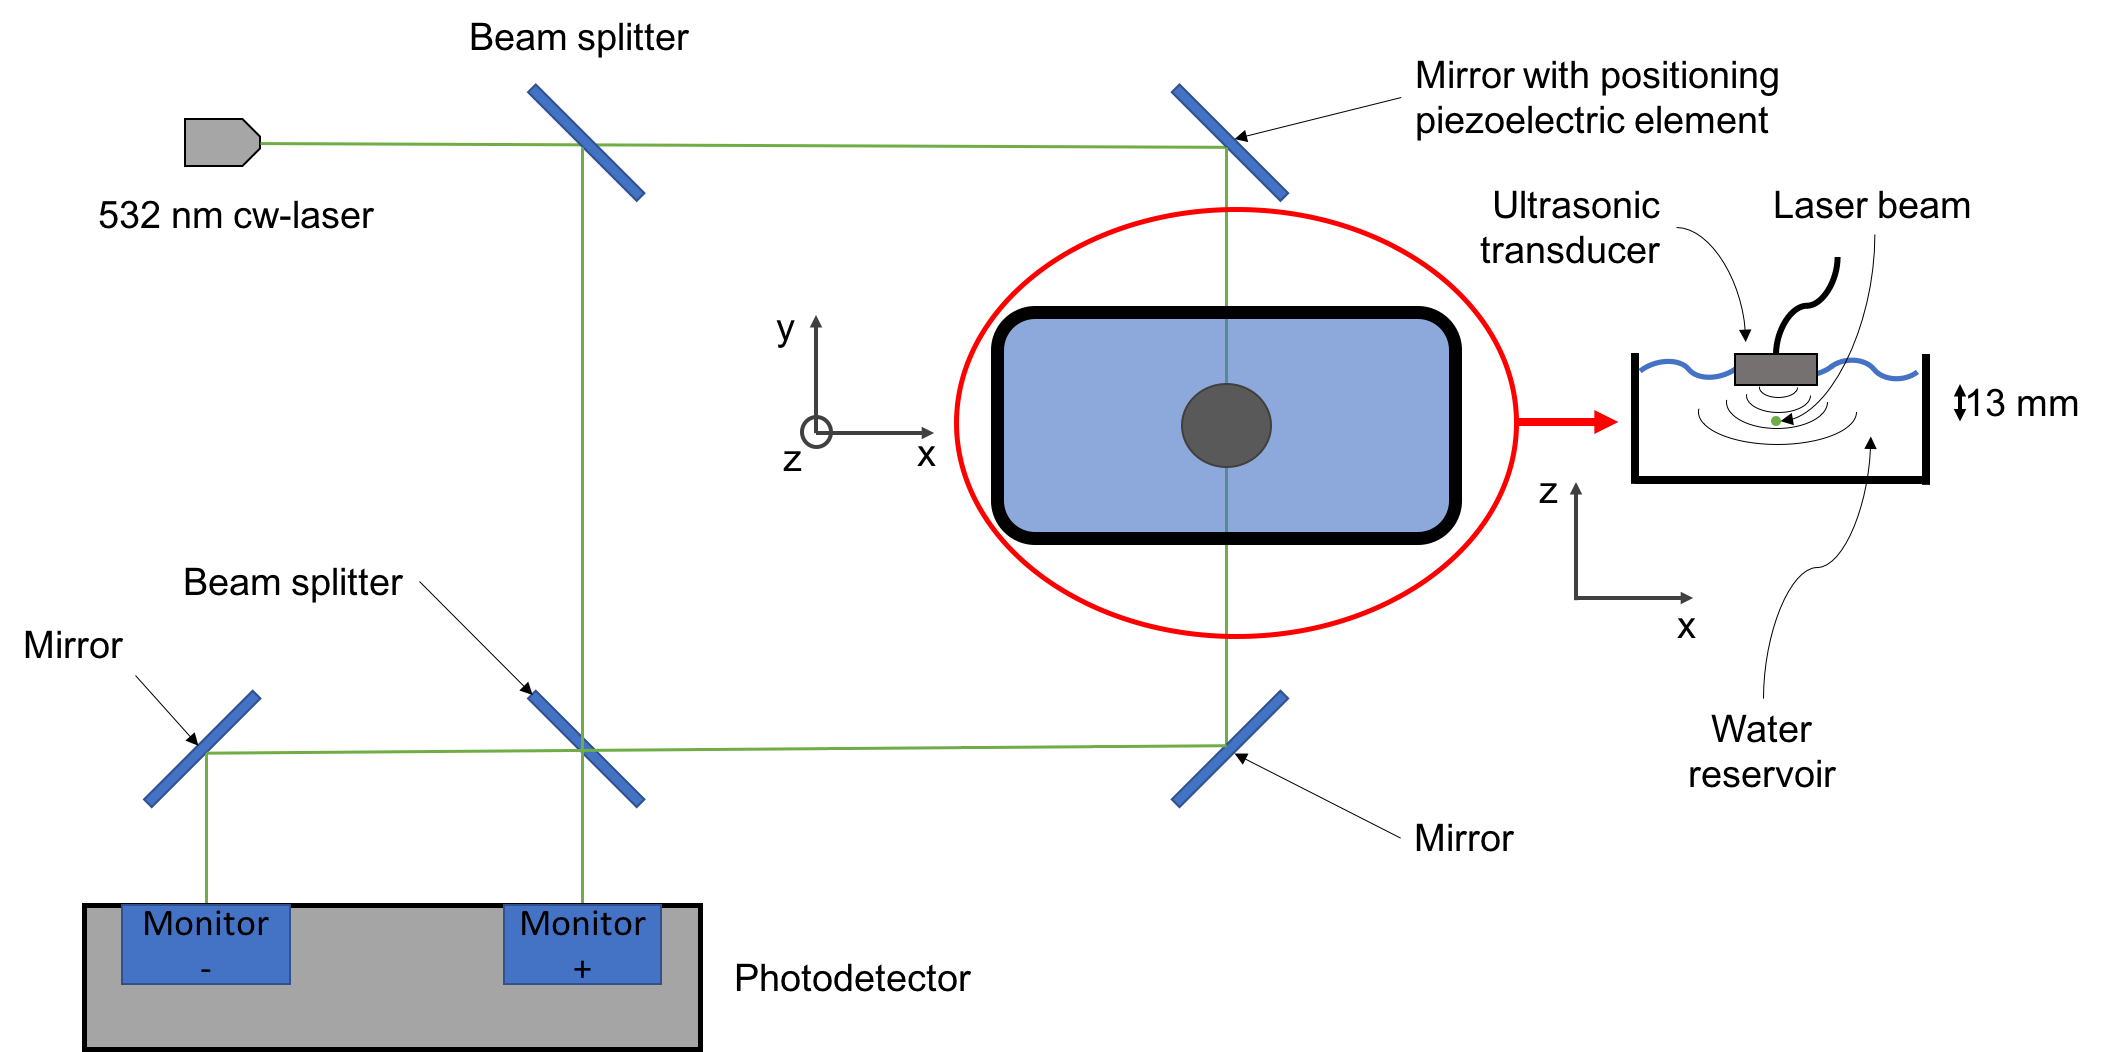
\includegraphics[height=0.4\textheight]{05_OUSD/images/MZinterSchem.png}
	\caption{Schematic of a Mach-Zehnder interferometer.}
	\label{fig:MZinterSchem}
\end{figure} 

A cw-laser with 532~$nm$ wavelength were split into two optical paths. The first one directly hits a second beam splitter and acts as a reference signal. The second one gets deflected by a mirror and guided through a water reservoir. Here the laser beam can interact with the ultrasonic wave of an ultrasonic transducer, which were also placed inside the reservoir. The distance in between were also chosen to be 13~$mm$. \\
Afterwards the second beam also hits the lower beamsplitter shown in figure \ref{fig:MZinterSchem}. The two beams then are guided towards a balanced amplified photodetector, PDB120A from Thorlabs, with two separate optical inputs.\\
If the water reservoir would not exist the intensity at the photodetector inputs "Monitor -" and "Monitor +" would follow the proportionality

\begin{equation}
I_- \sim \cos^2\left(\frac{\Phi}{2}\right) \; ;\; I_+ \sim \sin^2\left(\frac{\Phi}{2}\right) 
\label{eq:I+I-}
\end{equation}
\\
therefore a $\Delta\Phi = 0$ follows a maximum intensity at Monitor - and a minimum at Monitor +. The dependence of the phase shift between the two inputs is illustrated in figure \ref{fig:MZoutput}. 

\begin{figure}[H]
	\centering
	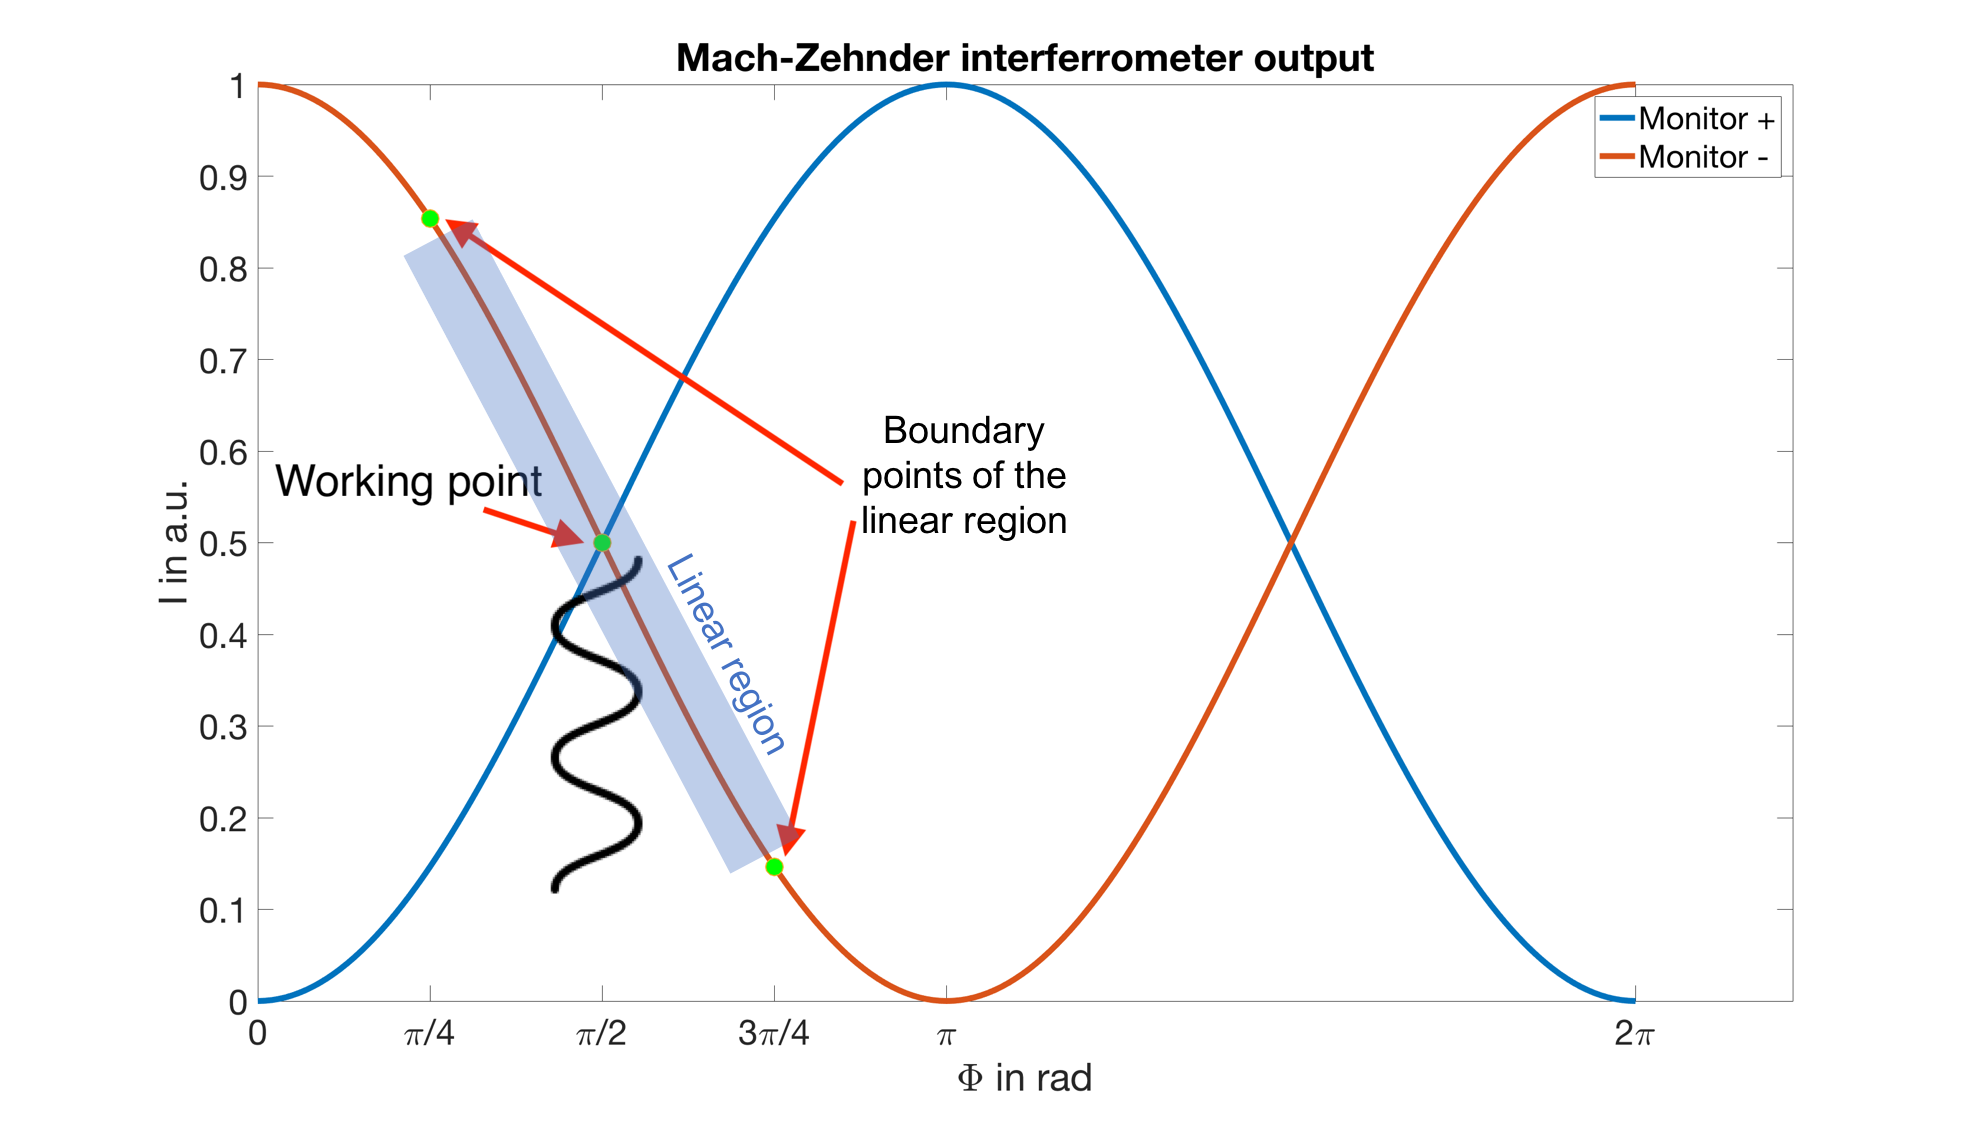
\includegraphics[height=0.4\textheight]{05_OUSD/images/MZoutput.png}
	\caption{Mach-Zehnder interferometer output function dependent on phase shift.}
	\label{fig:MZoutput}
\end{figure} 

In order to get the detector output signal shown in figure \ref{fig:MZoutput}, with the water reservoir inserted, a control loop were applied to the system. The operation point has to be in the steepest part of the linear region, shown in figure \ref{fig:MZoutput}. Therefore a mirror were mounted on a piezo transducer (upper right mirror in figure \ref{fig:MZinterSchem}) and used as an optical phase shifter.\\
Due to the refractive index of water changes in dependency to pressure, the phase between the optical paths of the Mach-Zehnder interferometer changes, too. This is given by

\begin{equation}
\Delta\Phi = k \cdot \frac{\partial n}{\partial p} \cdot \int_{0}^{L}p(x)\mathrm{d}x
\label{eq:MZphaseP}
\end{equation}
\\

there $k = \frac{2\pi}{\lambda}$ is the wave vector and $L$ is the interaction length. With the assumption that the incident pressure wave is a plane wave, as shown in figure \ref{fig:pInteract}, the pressure distribution over the interaction length  $L$ becomes constant.

\begin{figure}[H]
	\centering
	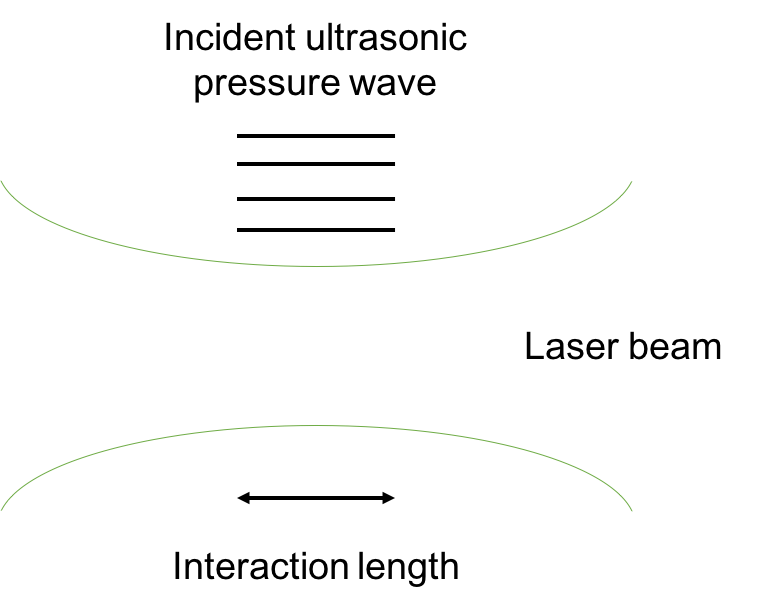
\includegraphics[width = 0.4\textwidth, height=0.2\textheight]{05_OUSD/images/pInteract.png}
	\caption{Schematic of the interaction between an ultrasonic pressure wave and laser beam.}
	\label{fig:pInteract}
\end{figure} 

Therefore equation \ref{eq:MZphaseP} reduces to 

\begin{equation}
\Delta\Phi = \frac{2\pi}{\lambda} \cdot \frac{\partial n}{\partial p} \cdot p \cdot L
\label{eq:MZphasePred}
\end{equation}
\\

The signal sequence shown in figure \ref{fig:MZoutput} is the light intensity that reaches the two optical photodetector inputs, but the measured voltage $U_s$ is the difference between Monitor - and Monitor +. This leads to 

\begin{equation}
\Delta\Phi \sim \frac{U_s}{2\cdot U_{cf}} 
\label{eq:MZpropUs}
\end{equation}
\\

there $U_s$ is the measured signal voltage, $U_{cf}$ is the conversion factor from light intensity to a voltage signal and the factor $2$ follows from the two inputs. \\
The working area of the intensity profile, shown in figure \ref{fig:MZoutput}, is the linear region of the $\sin^2(x)$ function and its range is $\frac{\pi}{2}$. Adding a modulation voltage $U_{mod}$ scaling follows

\begin{equation}
\Delta\Phi = \frac{U_s \cdot \pi}{4 \cdot U_{cf} \cdot c \cdot U_{mod}} 
\label{eq:MZeqUs}
\end{equation}
\\

there $c = 0.70711$ is the result of $c = \sin^2(\frac{3}{4}\pi) - \sin^2(\frac{1}{4}\pi)$ and defines the valid region of $U_{mod}$. Furthermore, $U_{mod}$ is the maximum voltage range of the photodetector output. The result of formula \ref{eq:MZphasePred} with formula \ref{eq:MZeqUs} and solving for $p$ follows

\begin{equation}
p = \frac{\lambda \cdot U_s}{16 \cdot U_{cf} \cdot c \cdot U_{mod} \cdot L \cdot \frac{\partial n}{\partial p}} 
\label{eq:MZp}
\end{equation}
\\

This formula converts the measured voltage signal $[V]$ into a equivalent pressure signal $[Pa]$. 







